\begin{abstract}
Retrieval-augmented generation systems increasingly detect contradictions among retrieved passages and flag them to
the generator. We ask what a flag must say, and how accurate its detector must be, to help against
misinformation. On fixed passages from five benchmarks, with seven generators from three families, we vary
detector and flag format, in hypotheses pre-registered (H1--H9 before any confirmatory data,
H10--H31 in eight later addenda). A perfectly accurate neutral flag (``these passages conflict'') does not reliably
help. Its effect depends on answer policy and model family; pooled over \neuMlK\ settings, allowing
for shared questions, it is \neuMlMu\ points \neuMlCI\ (exploratory). Naming the false side helps, but on average no more than
an answer key naming the wrong answer (pooled difference \PoolTwentyThree\ points, equivalent within $\pm$3 on average). In a
randomised test, a flag naming the false side raises accuracy by \hThirtyOneAMin\ to \hThirtyOneAMax\ points; naming the correct side lowers it by
\ahThirtyOneBMax\ to \ahThirtyOneBMin. Randomised flags on true pairs therefore help only above a break-even direction
precision, rising with generator accuracy from \beMin\ to \beMax. Real detectors are selective, so this
threshold alone can misjudge them. This test's follow rates, with each cell's coverage and no-flag
accuracy, account retrospectively for the flag's effect in \predEightN\ crossed detector--generator cells
($r=\predEightR$, mean error \predEightMae\ points; exploratory). What a
detector contributes is its verdict: passed as an answer key, it matches the flag (pooled, equivalent within $\pm$3). On genuine
conflicts, direction removes valid answers, and when conflicts are rare a real detector's false flags on clean
questions can outweigh its gains. We release the harness, pre-registrations and every run.
\end{abstract}
\section{Introduction}

Retrieval-augmented generation (RAG) \citep{lewis2020rag} hands a language model passages that may disagree. Some
disagreements are genuine; others are planted or stale misinformation \citep{zou2025poisonedrag,wang2025madam}. Recent systems pair contradiction detectors with prompts flagging conflicting passages
\citep{wang2026conflictrag}, and prompting a model about conflicts can help \citep{cattan2025conflicts}. They
report detection F1 and end-to-end accuracy but not how the two connect. What should the flag say, and what must the
detector get right for it to help?

We fix the passages and independently vary the \emph{detector} (heuristic, NLI, LLM, random placebo,
oracle, and synthetic detectors of chosen quality) and the \emph{format} passing its output to the generator: a
neutral ``these passages may conflict'' flag, a flag saying one side is false, not which, a
\emph{directional} flag naming the likely misinformation, or removal of the suspect passage. After pilots on
RAMDocs \citep{wang2025madam}, we pre-registered hypotheses H1--H9 and tested them on 300 held-out questions.
Eight addenda (H10--H31), each committed before its runs, extended the study to ConflictBank \citep{su2024conflictbank}
(including a majority-misinformation variant), to RAGuard \citep{zeng2025raguard}, whose
misleading side is real Reddit posts, and to seven generators from OpenAI, Anthropic and Qwen. Controls separate what a
flag conveys: forced choice, an answer key, randomised direction, the detector's verdict as an answer key and its model's own answer as
a hint, and \hTwentyFourCells\ cells crossing six detectors with six generators. WikiContradict \citep{hou2024wikicontradict}, whose conflicts are genuine, is the contrast case.

Our findings:
\begin{itemize}[leftmargin=*,itemsep=1pt,topsep=2pt]
\item \textbf{A correct neutral flag does not reliably help.} Asked for every valid answer, OpenAI and Qwen models also give the
misinformation; asked for one answer, some generators abstain on misinformed and correct answers
alike; under forced choice the effect is small. Claude models move less; the minimal prompt is most harmful.
These policy and family splits were coded after seeing data.
\item \textbf{An oracle's direction is a ceiling.} Naming the false side helps on every benchmark that labels one, but
on average it is equivalent to an answer key naming the wrong answer (pooled over \PoolTwentyThreeK\
comparisons, which vary individually).
\item \textbf{A directional flag pays only above a break-even precision.} When direction is randomised (H31), a wrong
flag costs more than a right one gains, because generators follow both at similar rates and an accurate generator has
more correct answers to lose. The break-even direction precision, which calibrates flags on true pairs, rises from \beMin\ for gpt-4o-mini to
\beMax\ for gpt-6.1-terra. For real detectors precision alone can mislead; the follow rates, with
what each detector flags, account for the effects (retrospective; Figure~\ref{fig:reliability}). The detector's verdict as an answer key matches its flag (H30); its model's
own answer as a hint does worse (H27).
\item \textbf{Direction is unsafe on genuine conflicts and costly when conflicts are rare.} On WikiContradict the LLM
directional flag and removal cut the share of answers giving both valid sides (H28); at a 5\% share of conflict
questions the LLM detector's flag has a negative estimated effect in \prevNegFive\ of \prevN\ settings (exploratory).
\end{itemize}
On CONFLICTS, the one benchmark of real search results, no condition changes accuracy significantly. We release the harness, pre-registrations and every run.\footnote{Code, the pre-registration and
all run outputs are in the anonymised supplementary material and will be released publicly on acceptance.}
\section{Related Work}
\label{sec:related}

\paragraph{Knowledge conflicts.}
Models can prefer memorised knowledge over contradicting context \citep{longpre2021entity}, yet coherent contradicting evidence
readily persuades them \citep{xie2024chameleon}, depending on their prior's strength \citep{wu2024clasheval}. \citet{huang2025trust} train models to decide whether to trust context or memory,
including real incorrect Reddit contexts. Context-faithful prompting changes how readily models follow
conflicting context or abstain \citep{zhou2023context}. Among the conflict types of \citet{xu2024survey}, we study inter-context
conflicts, as do \citet{chen2022rich}, who find models tend to rely on a single passage when evidence conflicts,
and \citet{wan2024convincing}, who find models weigh relevance over credibility cues.

\paragraph{Benchmarks.}
RAMDocs \citep{wang2025madam}, built on AmbigDocs \citep{lee2024ambigdocs}, mixes genuine ambiguity, misinformation
and noise. CONFLICTS \citep{cattan2025conflicts} annotates search results with conflict types and each type's
desired behaviour. WikiContradict \citep{hou2024wikicontradict} pairs genuinely contradicting Wikipedia passages.
FaithEval \citep{ming2025faitheval}, ConflictBank \citep{su2024conflictbank}, ConfRAG \citep{yuan2026confrag},
QACC \citep{liu2025qacc} and WhoQA \citep{pham2024whoqa} cover related settings. RAMDocs and ConflictBank label which side is misinformation; WikiContradict does not.

\paragraph{Telling the model about conflicts.}
Prompting a model to reason about the conflict type helps, and supplying the gold type helps much more
\citep{cattan2025conflicts}. On WikiContradict, models acknowledge both sides more often when told the passages may
conflict \citep{hou2024wikicontradict}. Ragability \citep{gross2026ragability} finds such a hint helps on
contradictory contexts but hurts on \emph{consistent} ones, where it is false. With our neutral flag the hint is
true and the input contradictory, yet accuracy falls: the hint does not say which side to trust.
RGB \citep{chen2024rgb} warns models that passages may contain errors, yet they rarely
detect them; our neutral flag is that warning, made pair-specific.
\citet{pan2023risk} test detection and ``vigilant'' prompting against LLM-generated misinformation, and
\citet{pan2023attacking} call for misinformation-aware QA. Source metadata and credibility signals also shape conflict resolution
\citep{chiang2024metadata,ge2025confact}.

\paragraph{Telling the model which passage is wrong.}
Closest to our directional format, \citet{hong2024gullible} pass a discriminator's marks on perturbed passages into the
generator's prompt, making the generator more robust to counterfactual noise. CrAM \citep{deng2025cram} rescales
attention by passage credibility, RA-RAG \citep{hwang2025rarag} estimates source reliability, and
\citet{weller2024defending} defend open-domain QA against disinformation. TACS \citep{yu2024tacs} detects untruthful context and masks it,
close to our removal. FaithfulRAG \citep{zhang2025faithfulrag} models
fact-level conflicts before generating. These works, with \citet{pan2023risk}'s finding that vigilant
prompts give limited protection, already show a reliability signal can help more than a warning; some vary
the signal's quality \citep{hong2024gullible,pan2024credibility}. Models also follow injected hints and asserted views, wrong
ones included \citep{turpin2023unfaithful,sharma2024sycophancy}. Advice improves a decision-maker only when its
errors fall where the decision-maker is less accurate \citep{bansal2021accurate,mozannar2020defer}, the
condition our break-even makes quantitative. Whether
abstaining is a failure depends on a wrong answer's cost \citep{wen2025abstention,song2025trustscore}.
We add a randomised direction manipulation on the same pairs, answer-key controls that separate the verdict
from the marking, its cost on clean questions, and a break-even direction precision per generator,
showing why it can misjudge selective detectors.

\paragraph{Detection, resolution and poisoning.}
ConflictRAG \citep{wang2026conflictrag} trains a pairwise detector with an LLM fallback and reports pair-level F1
alongside answer gains; its NLI and chain-of-thought baselines resemble two of our detectors. LLMs detect conflicts but struggle to pinpoint them
\citep{gokul2025contradiction,wang2024resolving,jiayang2024econ}. They favour the more frequent side, the side matching
their prior, and LLM-generated passages \citep{jin2024tugofwar,kortukov2024realistic,tan2024blinded}, and are
distracted by irrelevant context \citep{shi2023distracted,schuster2026whose}. TCR \citep{ye2026tcr}, context-aware
decoding \citep{shi2024cad}, EvidentialRAG \citep{hossain2026evidentialrag} and credibility-aware generation
\citep{pan2024credibility} learn or decode around unreliable passages. MADAM-RAG \citep{wang2025madam}, Astute RAG
\citep{wang2025astute}, Self-RAG \citep{asai2024selfrag}, Corrective RAG \citep{yan2024crag} and InstructRAG
\citep{wei2025instructrag} handle conflicts without an explicit detector. A few injected passages can steer a RAG
system \citep{zou2025poisonedrag}; RobustRAG \citep{xiang2024robustrag} isolates passages for certifiable robustness,
and TrustRAG \citep{zhou2025trustrag} filters suspected poisoned ones, the analogue of our removal. We ask instead how
to pass a detector's output to the generator.
\section{Framework}
\label{sec:method}

A question $q$ comes with retrieved passages $P=(p_0,\dots,p_{n-1})$. A \emph{detector} returns flagged pairs
$F\subseteq\{(i,j): i<j\}$; a \emph{directional} detector also returns, for each flagged pair, a \emph{suspect}
set $S_{ij}\subseteq\{i,j\}$: the side it believes is misinformation. A \emph{format} turns $(P,F,S)$ into the
generator's prompt. We vary detectors and formats independently. Every prompt shares a skeleton: passages, question,
and an instruction to end with a \texttt{Final answer(s):} line. The \emph{default} skeleton asks for every valid
answer when the passages support several (RAMDocs contains same-name ambiguity, so a correct answer may need several
entities). The \emph{minimal} skeleton drops that policy; its answer line allows several answers without inviting
them. The \emph{single} skeleton says the question has exactly one correct answer (true of ConflictBank by
construction). All three allow ``unknown'' when no passage answers the question; the \emph{forced} skeleton is
\emph{single} without that option (Appendix~\ref{app:prompts}).

\subsection{Formats}
\label{sec:formats}
\begin{description}[leftmargin=0pt,itemsep=1pt,topsep=2pt]
\item[No flags (plain).] Passages and question only.
\item[Instruction.] Plain plus a generic, detector-free instruction to check the passages for contradictions.
v1 ends ``if a disagreement reflects genuinely different valid answers, report each one''; v2 asks the model to
judge which passages are reliable and omit answers supported only by unreliable ones.
\item[Flag (neutral).] Each flagged passage gets the header \texttt{[POTENTIAL CONFLICT with passage(s): j]}, followed by a list
\texttt{Passages i and j: possible contradiction}. The format is CAAG's original, except that every detector's
flags render identically, so detectors differ only in \emph{which} pairs they flag.
\item[One-wrong flag.] As Flag, but adds that exactly one passage of the pair contains misinformation, without saying
which.
\item[Directional flag.] As Flag, but suspect passages are headed \texttt{[LIKELY MISINFORMATION; conflicts with
passage(s): j]}, and the list says which passage likely contains misinformation.
\item[Controls.] \emph{Pick}: the neutral flag plus ``decide which side is better supported and answer with that
side only''. \emph{No pairs}: flagged passages are marked, but not which conflicts
with which. \emph{Answer key}: plain plus ``The answer $X$ is false'' for each wrong answer, with no passage marked.
\item[Remove (suspect).] Each flagged pair's suspect passages are deleted. For a pair without a suspect, the
second passage is deleted, as the original CAAG \textsc{remove} strategy does without retrieval scores.
\item[Single call.] No detector: one call that writes \texttt{Suspect passages: \dots} and then answers from
the other passages, at half the calls of a detector pipeline.
\item[Closed book.] No passages: what the generator knows without retrieval.
\end{description}

\subsection{Detectors}
\label{sec:detectors}
\begin{description}[leftmargin=0pt,itemsep=1pt,topsep=2pt]
\item[CAAG] (Contradiction-Aware Attention Gating) is a heuristic detector from an earlier, unpublished RAG system,
used with its code unchanged. CAAG scores similar pairs by negation, entity-mismatch and temporal cues, runs locally
and gives no direction (Appendix~\ref{app:extra}).
\item[NLI] is \texttt{nli-deberta-v3-base} \citep{he2023debertav3}, a cross-encoder scored in both orders; a pair is
flagged if the larger contradiction probability exceeds $0.5$. It gives no direction.
\item[LLM] is a single call that lists, as JSON, contradicting pairs, distinguishing them from ambiguity, complementary and
temporal relations, and names the side more likely to be misinformation (or ``both'' or ``unclear''). It is
gpt-4o-mini (temperature 0) unless stated; in the crossed design gpt-4.1, gpt-6-luna, gpt-6.1-terra, Claude Haiku 5.5
and Claude Sonnet 5.5 run the same prompt.
\item[Random] flags each pair independently at CAAG's per-pair flag rate, a placebo.
\item[Oracle] flags exactly the gold contradiction pairs and names the gold misinformation side. The
\emph{inverted oracle}, an adversarial control, flags the same pairs but names the correct side.
\end{description}

\subsection{Synthetic detectors}
\label{sec:synthetic}
To separate a detector's accuracy from its identity, we build detectors from gold labels with a chosen pair-level
precision $p\in\{0.25,0.5,0.75,1\}$, recall $r\in\{0.25,0.5,1\}$ and direction accuracy $d\in\{0.5,0.75,1\}$ (36
grid cells), each rendered as a directional flag and as removal. All cells reuse the same random draws, so they are nested
and comparisons across cells are paired (Appendix~\ref{app:grid}).
\section{Experimental Setup}
\label{sec:setup}

\paragraph{Data.}
\textbf{RAMDocs} \citep{wang2025madam} has 500 questions, each with 1--12 documents (5.5 on average) typed
\emph{correct} (supports a gold answer, possibly for a different same-name entity), \emph{misinfo} (supports a wrong
answer) or \emph{noise}. A pair is a \emph{contradiction} if one side is misinformation and the answers differ,
\emph{ambiguity} if both are correct with different answers, \emph{consistent} if the answers match, and
\emph{unrelated} if either is noise. A \emph{conflict} question has a contradiction pair; a
\emph{clean} one has none. Some documents typed \emph{correct} contain a wrong answer; questions whose only sign of
conflict is such a document count only in ``All'' (Appendix~\ref{app:repro}).

\textbf{ConflictBank} \citep{su2024conflictbank}: for a Wikidata fact, an LLM writes one passage for the true
object and one for a substituted object. We sample 400 questions round-robin over relations: 300 conflict questions
(correct passage, misinformation passage, two distractors from other subjects) and 100 clean ones (correct passage,
three distractors). Every question has one gold answer. ConflictBank had no pilot: its registered tests come from the addenda (Table~\ref{tab:claims}), and everything else on it is exploratory. A
\emph{majority} variant gives each conflict question the correct passage and ConflictBank's three wrong-object
passages for that fact (its misinformation, temporal and semantic conflicts, all supporting the substituted object
and counted as misinformation), so the false side outnumbers the truth three to one.

\textbf{RAGuard} \citep{zeng2025raguard} pairs PolitiFact claims (true or false) with Reddit posts that an LLM
labelled supporting, misleading or unrelated, so the misleading side is real online text. We keep 294 claims with at
least one supporting and one misleading post (up to two of each, plus two unrelated posts) and 100 with no
misleading post; the question is whether the claim is true. Its post labels are behavioural: supporting or misleading according to whether GPT-4 judged the claim correctly with the post in context \citep[\S3.3]{zeng2025raguard}. They do not verify that two posts contradict or that the misleading one is false, so on RAGuard the ``oracle'' is a label transfer, not a factual oracle (audit in Appendix~\ref{app:semantic}).

\textbf{WikiContradict} \citep{hou2024wikicontradict} has 253 questions, each with two genuinely contradicting
Wikipedia passages; the reference answer is \emph{both} sides. The original evaluation also asks that an answer acknowledge the incompatibility and not prefer a side without support \citep[\S3.4]{hou2024wikicontradict}, so we measure coverage of the competing sources (original rubric in Appendix~\ref{app:semantic}). We also run 237 automatically scorable
\textbf{CONFLICTS} \citep{cattan2025conflicts} questions (Appendix~\ref{app:repro}).

\paragraph{Pre-registration and splits.}
We developed the method on a random 200-question RAMDocs pilot split. Before running anything on the remaining 300
questions (139 conflict, 126 clean, 35 excluded), we committed a pre-registration fixing the conditions, metrics,
hypotheses and corrections. These hypotheses, H1--H9, are the confirmatory core, registered before any confirmatory
data. Every RAMDocs result in the main text is on this confirmatory split; pilot results appear only in the appendix.
Unregistered comparisons, including every real-detector row of Table~\ref{tab:main}, are exploratory.
Eight addenda registered H10--H31, each committed before its runs, so these were formed after the
original confirmatory results were known. The last two addenda also registered re-analyses of data already
seen. A final round of re-analyses (pooled answer-key comparisons, break-even precision, the prediction of the crossed
cells, prevalence reweighting and a programme-wide FDR) was not registered. A ninth addendum (\S17) registered
further re-analyses, corrected baselines and a semantic re-score, after a mock review and before their runs. All of
these are exploratory (Table~\ref{tab:claims}). The repository's commit history is the only timestamp. Appendix~\ref{app:repro} lists every deviation.

\paragraph{Generators and baselines.}
The main generator is \texttt{gpt-4o-mini} \citep{openai2024gpt4o} (temperature 0.1, at most 256 output tokens, seeds
0--2). We replicate key conditions with \texttt{gpt-4.1}, Qwen2.5-7B-Instruct \citep{yang2024qwen25} (4-bit, local),
two reasoning models, \texttt{gpt-6-luna} (3 seeds) and \texttt{gpt-6.1-terra} (seed 0; one sample), and
Claude Haiku 5.5 (3 seeds) and Claude Sonnet 5.5 (seed 0). The reasoning and Claude models run at their default
temperature with up to 4,096 output tokens. On ConflictBank the primary prompt is
the single skeleton; the default and minimal skeletons are robustness checks. We rerun the oracle and LLM-detector
conditions with the minimal skeleton.
The LLM detector is gpt-4o-mini except in the crossed design (H24), where six detectors and six generators form
\hTwentyFourCells\ of the possible pairs on ConflictBank; we also run it on Qwen2.5-7B with gpt-4o-mini generating. Two controls test
whether a crossed cell's gain is only a stronger model's answer (H27): an own-answer hint (the detector model's plain
answer) and the detector model as the generator. An artefact probe (H29) reruns two detectors on
ConflictBank with passage order reversed and with every passage paraphrased by one model.
MADAM-RAG \citep{wang2025madam} is ported unchanged (three debate rounds). Astute RAG \citep{wang2025astute} and
TrustRAG \citep{zhou2025trustrag} use their published prompts and defaults; since both return one answer, we also run
\emph{multi} variants asking for every valid answer (Appendix~\ref{app:repro}). A detector pipeline counts as one
detector call plus one generator call.

\paragraph{Metrics.}
On RAMDocs an answer is correct if it includes every gold answer and no wrong answer \citep{wang2025madam}. Our primary
metric reads ``includes'' literally: after normalisation, each gold or wrong answer must be a whole-word span
of the extracted final answer. A bidirectional variant, which also counts a predicted answer contained in a gold one,
is the robustness metric: a result is \emph{robust} if it also holds under it. We chose the one-way metric before the confirmatory run because it is closer to MADAM-RAG's
published score (Appendix~\ref{app:repro}), and we compare conditions only within our harness. On WikiContradict
an answer is correct if it contains both sides (bidirectional matching); on ConflictBank and RAGuard we use the RAMDocs metrics. We also report
misinformation share (answers containing the misinformation), abstention share (``unknown'') and selective accuracy
(correct over answered). An LLM judge (gpt-6.1-terra) agrees with the primary metric on \judgeAgree\% of \judgeN\ stratified
conflict-question outputs ($\kappa=\judgeKappa$); the metric is slightly conservative, missing some paraphrases. We
release an unlabelled 200-output human-audit sheet.

\paragraph{Statistics.}
We average each question's score over seeds and report paired differences from the plain format, with
bootstrap 95\% CIs over questions (10,000 resamples) and two-sided sign-flip permutation tests
\citep{efron1993bootstrap,dror2018hitchhiker} (10,000 permutations, extended to 200,000 when none reaches the observed
statistic). A \emph{family} is the set of tests one hypothesis registers (e.g.\ H15 across generators). A registered
test takes its family's Holm-adjusted $p$ \citep{holm1979simple}. The \nExploratory\ exploratory comparisons of the
condition tables form one family, and the hypothesis tables add a Benjamini--Hochberg $q$ over all registered tests.
Only results significant under Holm are called significant or set in bold; CIs are unadjusted and not read as
significance. A null difference is not read
as equivalence without a TOST \citep{lakens2017equivalence} at $\pm$3 points. Selective accuracy is a ratio, tested by swapping conditions within questions. Pooled estimates use a multilevel model with random
effects for generator, benchmark and setting. Appendix~\ref{app:repro} gives the minimum detectable effect.

\paragraph{Cost.}
Token counts are from the API's usage reports. All experiments, pilots included, cost \totalSpend\ in API fees
(prices checked on 2026-10-27; Appendix~\ref{app:repro}).
\section{Results}
\label{sec:results}

Tables~\ref{tab:cb} and \ref{tab:main} give every condition and the hypothesis tables every registered test.
Table~\ref{tab:claims} marks each claim below as registered before any confirmatory data (H1--H9), in a later addendum before its
runs (H10--H31), or a re-analysis of data already seen (Appendix~\ref{app:extra});
Table~\ref{tab:evidence} says what each benchmark can support.

\subsection{What a neutral flag does depends on the answer policy}
\label{sec:neutral}
\begin{table*}[t]
\centering\small
\setlength{\tabcolsep}{3.5pt}
\resizebox{\textwidth}{!}{%
\begin{tabular}{lrrrrrrrrrrrr}
\toprule
& \multicolumn{4}{c}{No flags} & \multicolumn{4}{c}{Oracle, neutral flag} & \multicolumn{4}{c}{Oracle, directional flag} \\
\cmidrule(lr){2-5}\cmidrule(lr){6-9}\cmidrule(lr){10-13}
Generator & Correct & Misinfo. & Abstain & Sel. & Correct & Misinfo. & Abstain & Sel. & Correct & Misinfo. & Abstain & Sel. \\
\midrule
\multicolumn{13}{l}{\emph{RAMDocs, multi-answer prompt}} \\
gpt-4o-mini & 22.1 & 47.7 & 3.4 & 22.8 & 15.3 & \textbf{61.9} & 5.0 & 16.2 & 35.5 & \textbf{14.9} & 2.9 & \textbf{36.5} \\
gpt-6-luna & 14.4 & 72.2 & 1.2 & 14.6 & 11.3 & 76.7 & 0.7 & 11.4 & 53.5 & \textbf{11.3} & 1.4 & \textbf{54.3} \\
Claude Haiku 5.5 & 25.2 & 55.2 & 2.2 & 25.7 & 26.4 & \textbf{47.2} & 2.2 & 27.0 & 53.5 & \textbf{6.7} & 2.9 & \textbf{55.1} \\
gpt-6.1-terra & 10.8 & 75.5 & 2.2 & 11.0 & 10.1 & 81.3 & 1.4 & 10.2 & 50.4 & \textbf{13.7} & 2.2 & \textbf{51.5} \\
Claude Sonnet 5.5 & 45.3 & 24.5 & 2.2 & 46.3 & 45.3 & 21.6 & 2.2 & 46.3 & 59.7 & \textbf{3.6} & 1.4 & \textbf{60.6} \\
\midrule
\multicolumn{13}{l}{\emph{ConflictBank, multi-answer prompt}} \\
gpt-4o-mini & 21.6 & 72.8 & 0.3 & 21.6 & 12.8 & \textbf{83.2} & 0.9 & \textbf{12.9} & 49.4 & \textbf{41.2} & 1.2 & \textbf{50.1} \\
gpt-4.1 & 13.0 & 82.7 & 0.7 & 13.1 & 6.7 & \textbf{90.7} & 0.3 & \textbf{6.7} & 36.0 & \textbf{58.3} & 1.0 & \textbf{36.4} \\
Qwen2.5-7B & 23.7 & 67.0 & 6.0 & 25.2 & 15.3 & \textbf{79.0} & 5.0 & \textbf{16.1} & 41.3 & \textbf{52.0} & 13.0 & \textbf{47.5} \\
\midrule
\multicolumn{13}{l}{\emph{ConflictBank, one-answer prompt}} \\
gpt-4o-mini & 51.1 & 31.0 & 6.7 & 54.8 & 32.4 & \textbf{17.7} & \textbf{41.0} & 55.0 & 81.2 & \textbf{4.2} & \textbf{2.1} & \textbf{83.0} \\
gpt-6-luna & 53.6 & 24.3 & 11.9 & 60.8 & 44.1 & \textbf{17.4} & \textbf{28.9} & 62.0 & 90.0 & \textbf{0.0} & \textbf{0.8} & \textbf{90.7} \\
Claude Haiku 5.5 & 66.8 & 22.0 & 1.2 & 67.6 & 67.4 & 22.1 & 0.9 & 68.0 & 90.1 & \textbf{0.2} & 1.1 & \textbf{91.1} \\
gpt-6.1-terra & 73.0 & 18.0 & 1.7 & 74.2 & 70.7 & 15.7 & 4.7 & 74.1 & 90.0 & \textbf{0.7} & 0.3 & \textbf{90.3} \\
Claude Sonnet 5.5 & 75.7 & 15.7 & 1.0 & 76.4 & 78.7 & 12.0 & 1.7 & 80.0 & 92.0 & 1.0 & 1.7 & 93.6 \\
gpt-4.1 & 64.7 & 27.3 & 1.7 & 65.8 & 56.7 & 21.7 & 14.0 & 65.9 & 91.3 & 0.3 & 1.7 & 92.9 \\
Qwen2.5-7B & 50.3 & 35.3 & 5.0 & 53.0 & 47.0 & 28.7 & 15.0 & 55.3 & 75.7 & 13.0 & 1.3 & 76.7 \\
\midrule
\multicolumn{13}{l}{\emph{ConflictBank, forced choice}} \\
gpt-4o-mini & 55.4 & 31.6 & 0.1 & 55.5 & 55.2 & 31.9 & 0.4 & 55.5 & 79.7 & \textbf{6.7} & 0.0 & \textbf{79.7} \\
gpt-6-luna & 64.6 & 25.8 & 0.0 & 64.6 & 66.1 & 22.0 & 0.0 & 66.1 & 91.0 & \textbf{0.1} & 0.0 & \textbf{91.0} \\
Claude Haiku 5.5 & 69.3 & 20.9 & 0.0 & 69.3 & 73.2 & \textbf{16.8} & 0.0 & \textbf{73.2} & 90.4 & \textbf{0.0} & 0.0 & \textbf{90.4} \\
gpt-6.1-terra & 77.7 & 14.7 & 0.0 & 77.7 & 77.3 & 13.3 & 0.0 & 77.3 & 92.3 & \textbf{0.3} & 0.0 & \textbf{92.3} \\
\bottomrule
\end{tabular}}
\caption{Risk and coverage on conflict questions (\%): strictly correct answers, answers that contain the
misinformation, abstentions (``unknown''), and selective accuracy (correct answers over non-abstained answers, pooled
over questions and seeds). \textbf{Bold}: the change from no flags is significant (H21 for
ConflictBank one-answer and forced; the paper's exploratory family elsewhere). The answer policy decides what a neutral
flag does: under a prompt that asks for every valid answer it adds the misinformation to the answer; under a one-answer
prompt that allows ``unknown'' it moves answers, misinformed and correct, into abstention; under forced choice it has
no abstention to trade.}
\label{tab:risk}
\end{table*}


A neutral flag on exactly the gold contradictions lowers gpt-4o-mini's RAMDocs conflict-question accuracy
by \adOracleFlagConf\ points \dOracleFlagConfCI\ from \plainConf\% (H2), and gpt-4.1's by \agptOracleFlagConf\ (H9; Table~\ref{tab:risk} splits it by answer policy).

\paragraph{Asked for every valid answer, the model adds the misinformation.} Under RAMDocs' default prompt,
the flag raises gpt-4o-mini's
misinformation share from \zmRdMiniPlainWrong\% to \zmRdMiniOracleFlagWrong\%: told that two
passages conflict, it reports both sides. Every OpenAI and Qwen generator moves the same way; both Claude models
the other way (Haiku on RAMDocs \zmRdHaikuPlainWrong\% to \zmRdHaikuOracleFlagWrong\%).

\paragraph{Asked for one answer, it abstains.} Under the one-answer prompt, the
flag costs gpt-4o-mini \azSgMiniOracleFlagConflict\ points on ConflictBank, gpt-4.1 \azSgFourOracleFlagConflict\ and
gpt-6-luna \azSgLunaOracleFlagConflict\ (H15, H19), and changes accuracy insignificantly for gpt-6.1-terra,
Qwen2.5-7B, either Claude model (H25) and every generator on RAGuard (H26). Of gpt-4o-mini's misinformed answers, \trSgMiniNeutralMisinfoAbstain\% abstain with the flag and
\trSgMiniNeutralMisinfoCorrect\% become correct (\trNullSgMiniMisinfoCorrect\% between two unflagged seeds), and \trSgMiniNeutralCorrectAbstain\% of its
correct answers also abstain (H21). Under forced choice (H20), the flag has no
significant effect for gpt-4o-mini (\hTwentyFcMiniFlag), gpt-6-luna (\hTwentyFcLunaFlag) or gpt-6.1-terra
(\hTwentyFcTerraFlag), equivalence not established, and a small one for Claude Haiku (\hTwentyFcHaikuFlag).

\paragraph{Across settings.} In a multilevel model over the \neuMlK\ settings (Table~\ref{tab:pooled}; exploratory),
fitted with their sampling covariance (shared questions), the pooled effect is \neuMlMu\ points
\neuMlCI\ (\neuMlCIDesign\ conditional on these settings). A new setting would fall in \neuMlPI. The effect is
\neuPolMinimal\ \neuPolMinimalCI\ under the minimal prompt, \neuPolMulti\ under
multi-answer, \neuPolSingle\ under one-answer and \neuPolForced\ under forced-choice prompts, and Claude
shifts it up (\neuMlAnthropic; codings chosen after seeing data). If abstention is costless and a misinformed answer
costs $c$ wrong ones, the flag lowers utility significantly in \nUtilSixNegZero\ of \nUtilSixSettings\ settings at
$c=0$, and raises it in \nUtilSixPosFour\ at $c=4$ (Table~\ref{tab:utility}). On WikiContradict, where listing both valid sides is
correct, the flag raises accuracy (H8: \wikiOracleFlag).

\subsection{Naming the false side: what an oracle can deliver}
\label{sec:direction}
With the same oracle pairs, the directional flag beats the neutral and one-wrong flags in every registered comparison
but one (H3, H9--H12, H15, H16, H19, H25, H26; gpt-6.1-terra on RAGuard is not significant). On ConflictBank's
one-answer prompt it gains \azSgTerraOracleFlagDirectionalConflict\ to \azSgLunaOracleFlagDirectionalConflict\
points for the OpenAI generators and \azSgSonnetOracleFlagDirectionalConflict\ to
\azSgHaikuOracleFlagDirectionalConflict\ for Claude. It also helps under forced choice (H20) or majority
misinformation, and on RAGuard (H26). On RAMDocs it gains \adOracleDirConf\ points with gpt-4o-mini and
up to \azRdTerraOracleFlagDirectionalConflict\ with gpt-6.1-terra, but not significantly for Qwen2.5-7B or for
gpt-4o-mini under the minimal prompt (H10). The one-wrong flag helps only under forced choice (H16, H20).

Oracle rows are a ceiling, not a detector result. An answer key (``the answer $X$ is false'', no passage
marked) does as well: no registered comparison differs significantly (H23; \keyDiffMin\ to \keyDiffMax\ points).
Pooled over the \PoolTwentyThreeK\ comparisons (bootstrapping each benchmark's questions
jointly across them), the flag's advantage is \PoolTwentyThree\ points \PoolTwentyThreeCI, equivalent within $\pm$3 on average
(90\% CI \PoolTwentyThreeCINinety; exploratory). Individually, equivalence holds in only \hTwentyThreeEqN\ of
\hTwentyThreeK\ comparisons (SD \hTwentyThreeTau\ points between them). An inverted oracle
costs \aadvDirConf\ points on RAMDocs (Table~\ref{tab:inverted}).

\subsection{With a real detector, its wrong flags decide}
\label{sec:real}
\paragraph{Registered results differ by generator.} With the gpt-4o-mini LLM detector, the directional flag significantly raises
accuracy over all ConflictBank questions for \nRealSgPos\ of \nRealSgTests\ generators (gpt-6-luna,
\zSgLunaLlmDirFlagDirectionalLabelled) and significantly lowers it for \nRealSgNeg\ (gpt-6.1-terra,
\zSgTerraLlmDirFlagDirectionalLabelled; H15, H19, H25). It helps all \nRealMjTests\ generators under majority
misinformation (\zMjMiniLlmDirFlagDirectionalConflict\ to \zMjTerraLlmDirFlagDirectionalConflict), and on RAGuard the
two Claude models (H26: \hTwentySixRgHaikuLlm, \hTwentySixRgSonnetLlm) but no OpenAI one.

\begin{figure}[t]
\centering
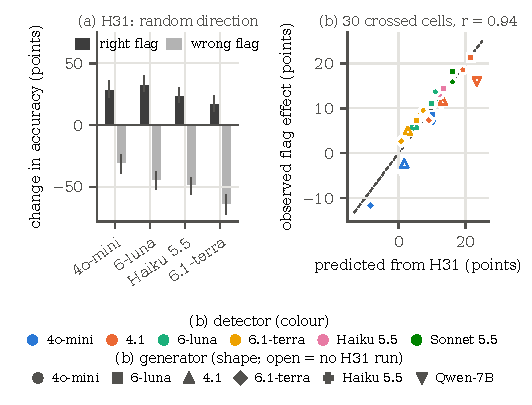
\includegraphics[width=\columnwidth]{generated/fig_reliability.pdf}
\caption{Left: randomised direction (H31; ConflictBank, one-answer prompt): change in accuracy (95\% CIs) on
conflict questions given a right flag (naming the false side) or a wrong flag (naming the correct side). Right: predicted (from H31's follow rates) against observed effect in the \predAllN\ crossed detector--generator
cells (filled: the generator's own rates; open: mean rates, for generators
with no H31 run); dashed: $y=x$. Exploratory and retrospective: the account was defined after the cells
(Table~\ref{tab:cells}) were seen.}
\label{fig:reliability}
\end{figure}
\paragraph{A wrong flag costs more than a right one gains.} In a randomised test (H31), each ConflictBank conflict
question was flagged on its true contradiction, naming the false side for a random \nRandRight\ and the
correct side for the other \nRandWrong. A right flag raises accuracy by \hThirtyOneAMin\ to \hThirtyOneAMax\ points and
a wrong one lowers it by \ahThirtyOneBMax\ to \ahThirtyOneBMin\ (Figure~\ref{fig:reliability}, left). The net effect is
significantly negative for \nHThirtyOneCSig\ of \nHThirtyOneCTests\ generators at an even mix (H31c) and for
\nRealThirtyOneSig\ at the split as run (\shareRight\% right; gpt-6-luna \realThirtyOneLuna\ \realThirtyOneLunaCI).
For right- and wrong-flag effects $R$ and $W$, randomised flags on true pairs do net harm below a break-even
direction precision $p^\star=-W/(R-W)$: \beMini\ \beMiniCI\ for gpt-4o-mini, \beLuna\ for gpt-6-luna, \beHaiku\ for Claude
Haiku and \beTerra\ \beTerraCI\ for gpt-6.1-terra (Table~\ref{tab:breakeven}; exploratory). Right- and wrong-flag
follow rates overlap (descriptive; Table~\ref{tab:breakeven}) except gpt-6.1-terra's, so $p^\star$ rises mainly
because an accurate generator has more to lose. This threshold is a calibration, valid for a real detector only if
it flags typical questions and nothing else.

\paragraph{Real detectors are selective.} Across H24's \hTwentyFourCells\ cells
(Table~\ref{tab:selection}), comparing precision with $p^\star$ can mislead. The gpt-4o-mini detector's precision
(\selHaikuMiniPrec\%) is just above Claude Haiku's break-even, implying \selHaikuMiniMarg\ points, but the cell's effect is
\selHaikuMiniObs: its flags on a correct passage (\selHaikuMiniWrongShare\% of questions) change accuracy there by
\selHaikuMiniWrongGain. The follow-rate account
$\hat\Delta=\frac1n\sum_i[d_i(1-a_i)f_R-w_ia_if_W]$ is a retrospective decomposition, defined after the cells were
seen ($d_i$: the flag
names the false side; $w_i$: it marks a correct passage; $a_i$: no-flag accuracy; $f_R,f_W$: H31's follow rates). The
account tracks the \predEightN\ cells with an H31 generator
($r=\predEightR$ \predEightRCI, mean error \predEightMae\ points, against \predGenMae\ for each generator's mean over
its other cells; $r=\predXfR$ with no-flag answers from another seed), mostly through the cell-level rates
(\predMargMae\ with cell means alone), but misses the Haiku cell (\predHaikuMini). The registered H24 correlation is uninformative, since generator accuracy
enters both sides. The least precise detector (gpt-4o-mini, \dirPrecMini\%) lowers accuracy for the four most
accurate generators, significantly for gpt-6.1-terra (H19).

\paragraph{What the detector contributes is its verdict.} The detector's judgement, passed as an answer key (``the
answer $X$ is false'' for the answer its suspect passage supports), matches the directional flag
(H30: \hThirtyAMin\ to \hThirtyAMax\ points per cell, none significant; pooled over the \PoolThirtyAK\ cells the flag
is ahead by \PoolThirtyA\ \PoolThirtyACI, equivalent within $\pm$3) and beats the detector model's own answer as a
hint by \PoolThirtyB\ \PoolThirtyBCI. That hint does worse than the flag in \nHTwentySevenAPos\ of
\nHTwentySevenATests\ cells and never better (H27).

\paragraph{With rare conflicts, false flags can outweigh gains.} The LLM detector also flags clean questions
(\cleanFprLlm\% of RAMDocs'). At a 5\% share of conflict questions its flag's estimate is negative in \prevNegFive\ of \prevN\ correlated settings
(bootstrap \prevNegFiveCI; significantly in \prevSigNeg, positive in \prevSigPos; Table~\ref{tab:prevalence}).

\paragraph{Genuine conflicts and baselines.} Reordering \citep{liu2024lost} or paraphrasing passages does not significantly
change the detectors' hit rate (H29). Where both sides are valid, direction does damage (H28): on WikiContradict the LLM directional
flag lowers the share of answers giving both sides by \ahTwentyEightWcMiniDir\ to \ahTwentyEightWcLunaDir\ points
(and of answers correct under the benchmark's own rubric by \awikiOrigMiniEffPt\ to \awikiOrigLunaEffPt;
Appendix~\ref{app:semantic}). On RAMDocs' same-name questions, removal costs every generator
\ahTwentyEightAmbMiniRem\ to \ahTwentyEightAmbLunaRem\ points. Against published defences, with answer policies matched and TrustRAG's
system message restored, the LLM directional flag beats TrustRAG by \blHFourteenCbs\ points on ConflictBank and
\blHFourteenRd\ on RAMDocs, but not under majority misinformation (\blHFourteenMj). The registered H14, with
mismatched policies, shows no win (Appendix~\ref{app:extra}).
\section{Discussion}
\label{sec:discussion}

A neutral flag leaves the model to its answer policy, so it suits only a one-answer policy with a measured cost for
wrong answers \citep{wen2025abstention}. A directional flag is advice generators follow whether
right or wrong, as with sycophancy \citep{sharma2024sycophancy}. Such advice pays only above a break-even precision, as in
human--AI complementarity \citep{bansal2021accurate,mozannar2020defer}. That threshold calibrates randomised flags on
true pairs; a selective detector needs its own test, which we did not run.
\section*{Limitations}

\paragraph{Models and detectors.} We test seven generators from three families: four OpenAI models (gpt-4o-mini,
gpt-4.1 and two current reasoning models), Claude Haiku 5.5 and Sonnet 5.5, and a 4-bit Qwen2.5-7B. Gemini
serves only as a judge, and we run no large open model. Qwen2.5-7B, gpt-6.1-terra and Claude Sonnet ran with one seed,
as did gpt-4.1 outside RAMDocs. The reasoning and Claude models ran only at default temperature and so sample
nondeterministically. Claude ran through Anthropic's OpenAI-compatible endpoint. The LLM detector is a single
prompt. The published baselines are reimplemented (Astute RAG has no official code; restoring TrustRAG's system message
changed little), NLI sees only a sentence-sized window, and we compare against no trained detector such as
ConflictRAG's \citep{wang2026conflictrag}. The crossed reliability test (H24) covers \hTwentyFourCells\
detector--generator cells on one benchmark with six detectors, so a test of a detector-level property has little
power (an exact permutation has \hRedoNPerm\ arrangements). The generator's own accuracy dominated the
registered H24 correlation. Concurrent runs gave a detector slightly different outputs across cells, but identical
ones for at least \frozenShareMin\% of questions; restricting each cell to those moves no
cell's gain by more than \frozenMaxShift\ points. The follow-rate account of the crossed cells was defined after seeing
them, using follow rates from the same questions, so it is a retrospective decomposition; no outcome-blind
question set tests it. The break-even precision is a calibration for randomised flags on true pairs, not a validated
rule for selective detectors.

\paragraph{Data and power.} Confirmatory evidence comes from two benchmarks: RAMDocs (300 questions, 139
with conflicts) and ConflictBank (400 sampled questions, 300 with conflicts). In both, misinformation is
synthetic, made by editing or generating text around a substituted answer; ConflictBank's passages are LLM-written
on both sides. The current reasoning models distrust ConflictBank's generated passages when asked to judge them
(Appendix~\ref{app:more}), which suggests generated benchmarks may not measure how such models treat real
documents. Reversing and paraphrasing the passages do not significantly change the detectors' hit rate (H29), but
equivalence within $\pm$5 points is shown for only one of four changes. Position, surface style and deeper regularities of generated text are therefore
not ruled out as sources of their direction. The majority variant tests one
case where the false side is more numerous, but its extra wrong-side passages are generated for the same substitution,
which a real attacker would vary, and include ConflictBank's temporal and semantic conflicts, which we count as
misinformation. RAMDocs' document labels are imperfect. We exclude 35 hold-out questions whose status depends on
documents we could not label without human annotation, and check that conclusions survive treating those
documents as misinformation. RAGuard's misleading side is real text, but its labels are behavioural (whether GPT-4
judged the claim correctly with the post). An LLM audit finds only \rgAudContradict\% of sampled supporting--misleading
pairs to contradict (Appendix~\ref{app:semantic}), so its oracle is a label transfer, not a factual oracle. With
posts in context, generators abstain on \rgAbstMin--\rgAbstMax\% of conflict claims, so accuracy on this
true/false task falls below chance; on the claims they answer it is \rgAnsMin--\rgAnsMax\%, against
\rgCbMin--\rgCbMax\% closed-book. Every generator is more accurate closed-book than with RAGuard's posts
(gpt-4o-mini \zcRgMiniConflict\% against \zpRgMiniConflict\%), so they make a weak retrieval setting.
WikiContradict has genuine conflicts but no misinformation side. CONFLICTS shows no significant effect for any
condition; scored only on items with a reference answer, it can neither confirm nor refute our findings. Our
comparisons detect effects of about \mdeMed\ points with 80\% power, so smaller effects, including small harms on clean
questions, may be missed.

\paragraph{Metric.} RAMDocs ships no scorer. Our primary metric reconstructs the published definition and scores our
MADAM-RAG port close to the published number on the pilot split, but the published subset is unknown, so this
is not a reproduction. The metric is string matching: it misses paraphrases, and partial answers interact with ``no wrong
answer''. We report the more lenient bidirectional variant throughout and mark conclusions that depend on
it. An outside-family LLM judge agrees with the matcher on \semAgree\% of \semN\ paired outputs. The matcher's
misses depend on the condition (more under answer keys and directional flags) but move no contrast by more than
\semDidMax\ points (Appendix~\ref{app:semantic}). That sample cannot confirm the $\pm$3-point equivalence claims, and
no human labels check either scorer: the paired, blinded audit sheet we release is unlabelled.

\paragraph{Direction and the grid.} Oracle direction is not distinguishable from an answer key (H23), so the
oracle rows are ceilings, not findings about detectors. Direction precision is the share of a detector's flags on true
contradictions that name the false side; pair precision, the share of its flagged pairs that are
true contradictions. The gpt-4o-mini LLM detector's direction precision is
\dirAccLlm\% on RAMDocs and \cbDirAccLlm\% on ConflictBank. Its per-question hit rate is lower because it also misses pairs. Its directional flag's gain over
all ConflictBank questions with gpt-4o-mini is not significant after correction (H15), and with stronger generators it
hurts. In the grid the gain rises with direction accuracy, but the grid cannot separate adjacent levels.
Synthetic false flags are spread uniformly with a random suspect side, whereas real detectors concentrate their
errors. The grid predicts real detectors only roughly, and three detectors cannot show whether document- or pair-level
summaries predict better.

\paragraph{Pre-registration.} H1--H9 were registered before the confirmatory run. H10--H31
were registered in eight addenda, after earlier results were known but before their own runs. The only
timestamp is the repository's commit history, not a third-party registry. Holm controls error within each family, not
across the programme: of \fdrN\ registered tests, \fdrHolm\ are significant under Holm and \fdrBH\ under a
Benjamini--Hochberg FDR over all of them (both in the hypothesis tables). Several analyses were chosen after
seeing data and are labelled as such: the TOST margin, the single- and multi-answer split, the document-level
placement axes, the post-hoc comparison of detector and generator reliability that H24 later tested, H24's mechanism
score, and the refinement of permutation $p$-values at their floor.

\paragraph{Scope.} We study flags passed to the generator as text. Learned interfaces such as soft prompts or
credibility fine-tuning \citep{ye2026tcr,pan2024credibility}, and retrieval-side filtering, may trade off differently. We test one adversarial case, a detector that always names the wrong side, not an attacker who controls
which pairs are flagged.

\section*{Ethics Statement}
This work uses public benchmarks and commercial model APIs, and involves no human subjects or personal data. Its main
risk is dual use: a false ``likely misinformation'' label, or removing a passage, can
change a RAG system's answers. An inverted oracle that names the correct side as misinformation costs \aadvDirConf\
points on RAMDocs and \azCbMiniOracleInvFlagDirectionalConflict\ on ConflictBank as a flag, and \aadvRemConf\ on
RAMDocs when the passage it names is removed. An adversary who can trigger a deployed detector could exploit this
\citep{zou2025poisonedrag}. We therefore report harm on clean questions alongside every gain, and argue that
systems should measure what a detector does at the document level before acting on its flags.
\section{Prompts}
\label{app:prompts}
The prompts below are verbatim from the code that produced the results. The examples use placeholder passages; in the runs every condition except removal shows the generator the same passages (checked against the run records).
\paragraph{Generation skeleton.}
\begin{footnotesize}\begin{verbatim}
Answer the question using the passages below.
If the passages support more than one valid answer
(for example, different people or things share the
same name), give every valid answer.
If no passage answers the question, the answer is
"unknown".
{instruction}
{context}
{conflicts}
Question: {question}

Give a brief explanation, then end with one line in
exactly this format:
Final answer(s): <answer 1> | <answer 2> | ...
\end{verbatim}\end{footnotesize}
\paragraph{Instruction v1.}
\begin{footnotesize}\begin{verbatim}
Some passages may contradict each other. Before
answering, check whether they do.
Ignore passages that appear to contain
misinformation, and if a disagreement reflects
genuinely different valid answers, report each one.
\end{verbatim}\end{footnotesize}
\paragraph{Instruction v2.}
\begin{footnotesize}\begin{verbatim}
Some passages may contain false information. Before
answering, decide which passages are reliable by
checking them against each other.
Do not include an answer that is supported only by a
passage you judge to be unreliable.
\end{verbatim}\end{footnotesize}
\paragraph{Example: directional flag (passage 2 suspect).}
\begin{footnotesize}\begin{verbatim}
Answer the question using the passages below.
If the passages support more than one valid answer
(for example, different people or things share the
same name), give every valid answer.
If no passage answers the question, the answer is
"unknown".

Passage 0 [POTENTIAL CONFLICT with passage(s): 2]:
<passage 0>

Passage 1:
<passage 1>

Passage 2 [LIKELY MISINFORMATION; conflicts with
passage(s): 0]:
<passage 2>

POTENTIAL CONFLICTS DETECTED:
- Passages 0 and 2: possible contradiction; passage
2 likely contains misinformation

Question: Who founded X?

Give a brief explanation, then end with one line in
exactly this format:
Final answer(s): <answer 1> | <answer 2> | ...
\end{verbatim}\end{footnotesize}
\paragraph{Directional LLM detector.}
\begin{footnotesize}\begin{verbatim}
You will see a question and {n} numbered passages
retrieved for it.
Some passages may contain misinformation: false
claims about the answer to the question.
Identify every pair of passages that CONTRADICT each
other about the answer to the question,
i.e. they cannot both be true about the same entity
at the same time. Passages that are about
different entities with the same name, give
complementary details, or describe different times
are NOT contradictions; note them as "ambiguity",
"complementary" or "temporal" instead.

For each contradiction, say which passage of the
pair is more likely the misinformation, judging
by agreement with the other passages and by
plausibility: its number, "both" if both are likely
false, or "unclear" if you cannot tell.

Question: {question}

{passages}

Return JSON only: {{"pairs": [{{"i": <int>, "j":
<int>, "relation":
"contradiction|ambiguity|complementary|temporal",
"misinformation": <int>|"both"|"unclear"}}]}}
Use the passage numbers shown. "misinformation" is
needed only for contradictions. Return {{"pairs":
[]}} if there are none.
\end{verbatim}\end{footnotesize}


\section{Additional Results}
\label{app:extra}

\paragraph{Published baselines (H14).} Astute RAG \citep{wang2025astute} and TrustRAG \citep{zhou2025trustrag} lose same-name answers
on RAMDocs (H14). On ConflictBank, the registered H14 compared our pipeline under the multi-answer prompt with the
baselines' own one-answer prompts. Under the matched one-answer prompt, which we take as the principal comparison, our pipeline beats them by
\hFourteenMatchedAst\ and \hFourteenMatchedTr\ points (exploratory). Our TrustRAG port
first omitted the repository's system message; sending it (\S17.2) changes TrustRAG's accuracy by \blTrustSysCb\
points on ConflictBank, \blTrustSysMj\ under majority misinformation and \blTrustSysRd\ on RAMDocs (\blTrustSysRdMulti\
for its multi-answer variant). Against the corrected TrustRAG, with policies matched (Holm over the four), the LLM
directional flag changes accuracy by \blHFourteenCbs\ on ConflictBank (one-answer), \blHFourteenRd\ on RAMDocs (multi-answer),
\blHFourteenMj\ under majority misinformation, and \blHFourteenCb\ under the registered mismatched prompts.
NLI on ConflictBank first saw passage prefixes that usually omit the changed fact. Cutting each passage to its
sentences closest to the question, up to the registered 1,500 characters, includes both answers, but the
pair still exceeds the cross-encoder's 512 tokens, and NLI flags no pair (pair recall \detNliWinRecall\%). With
300 characters, about one sentence (a disclosed deviation, \S17.6), NLI finds \detNliSentRecall\% of the gold pairs at
\detNliSentPrec\% pair precision and flags \detNliSentCleanFpr\% of clean questions. Its flag changes conflict
accuracy by \blNliSentFlag\ points (removal: \blNliSentRem). A single call that names suspect passages before
answering does not differ significantly from the pipeline (H18; Table~\ref{tab:baselines}).

\paragraph{Robustness to the metric and the labels.}
Table~\ref{tab:main_robust} repeats Table~\ref{tab:main} with the bidirectional metric, and Table~\ref{tab:contains}
repeats the pre-registered tests treating every suspect document as misinformation. Table~\ref{tab:hypotheses}
lists all pre-registered tests.

\begin{table*}[t]
\centering\footnotesize
\setlength{\tabcolsep}{4pt}
\begin{tabular}{p{7.4cm}p{3.6cm}p{4.2cm}}
\toprule
Claim (section) & Evidence & Status \\
\midrule
A correct neutral flag lowers RAMDocs accuracy (\S\ref{sec:neutral}) & H2, H9 & registered before any confirmatory data \\
Its mechanism depends on the answer policy: added misinformation, abstention, little effect (\S\ref{sec:neutral}) & Table~\ref{tab:risk}; H15, H19--H21, H25, H26 & answer mix: re-analysis; tests: registered addenda \\
Pooled effect, policy split, moderators, utility, transitions (\S\ref{sec:neutral}) & Tables~\ref{tab:pooled}, \ref{tab:utility} & re-analysis of data already seen; dependence: \S17 \\
The directional flag beats the neutral one (\S\ref{sec:direction}) & H3, H9--H12, H15, H16, H19, H25, H26 & H3: before any confirmatory data; rest: addenda \\
Oracle direction is close to an answer key (\S\ref{sec:direction}) & H23 and its TOST & registered addendum; TOST registered in \S13.4 \\
Pooled, oracle direction is equivalent to an answer key on average (\S\ref{sec:direction}) & pooled H23; per-comparison TOST & unregistered re-analysis; heterogeneity: \S17 \\
Real-detector gains depend on the generator (\S\ref{sec:real}) & H15, H17, H19, H25, H26 & registered addenda \\
Right flags gain less than wrong flags cost; similar follow rates (\S\ref{sec:real}) & H31 & registered addendum (\S16) \\
Break-even direction precision rises with generator accuracy (\S\ref{sec:real}) & Table~\ref{tab:breakeven} & unregistered re-analysis \\
Break-even is a calibration, not a rule for selective detectors (\S\ref{sec:real}) & Table~\ref{tab:selection} & re-analysis (\S17) \\
Follow rates and coverage account for the crossed cells (\S\ref{sec:real}) & Figure~\ref{fig:reliability} & unregistered; retrospective \\
Registered reliability gap correlates with the gain (\S\ref{sec:real}) & H24 & registered addendum (\S13), 5 of 30 cells existed \\
The gap is dominated by generator accuracy; precision and recall matter within generators (\S\ref{sec:real}) & Table~\ref{tab:h24redo} & re-analysis of data already seen \\
The detector's verdict as an answer key matches the flag; its model's answer as a hint does not (\S\ref{sec:real}) & H30, H27 & registered addenda (\S15, \S16); pooled TOST unregistered \\
A real detector's flag hurts when conflicts are rare (\S\ref{sec:real}) & Table~\ref{tab:prevalence} & unregistered re-analysis \\
Direction survives reordering and paraphrase (\S\ref{sec:real}) & H29 & registered addendum; equivalence not shown \\
Direction and removal harm genuine conflicts (\S\ref{sec:real}) & H28 & registered addendum \\
The matcher's errors do not change the contrasts' signs (App.~\ref{app:semantic}) & Table~\ref{tab:semantic} & registered re-score (\S17), LLM judge \\
Recommendations (\S\ref{sec:discussion}) & -- & not tested end to end \\
\bottomrule
\end{tabular}
\caption{The status of each claim. \emph{Registered addendum}: committed before the runs it covers but
after earlier results were known. \emph{Re-analysis}: registered after the data were seen, or exploratory. The commit
history is the only timestamp.}
\label{tab:claims}
\end{table*}

\begin{table*}[t]
\centering\footnotesize
\setlength{\tabcolsep}{4pt}
\begin{tabular}{p{2.3cm}p{3.6cm}p{4.4cm}p{4.6cm}}
\toprule
Benchmark & Misinformation and labels & What it supports & What it cannot support \\
\midrule
RAMDocs & synthetic edits; document labels imperfect & neutral and directional flags (H1--H12); confirmatory split & natural misinformation \\
ConflictBank & LLM-written on both sides; one gold answer & answer policy, randomised direction and break-even (H31), crossed cells (H24, H30) & real documents; prospective test of the cell account \\
RAGuard & real posts; behavioural labels (App.~\ref{app:semantic}) & what generators do with transferred labels & factual-oracle conclusions \\
WikiContradict & genuine conflicts, no false side & coverage of competing sources, and its original rubric (H28) & which answer is factually wrong \\
CONFLICTS & real search results; scorable subset & null results only & any positive claim \\
\bottomrule
\end{tabular}
\caption{The evidence hierarchy. The break-even precision rests on
ConflictBank alone; the other benchmarks add breadth for the flag-format results, not independent confirmations of it.}
\label{tab:evidence}
\end{table*}

\begin{table}[t]
\centering\small
\setlength{\tabcolsep}{4pt}
\begin{tabular}{@{}>{\raggedright\arraybackslash}p{3.3cm}rr@{}}
\toprule
Inverted oracle (names the correct side) & Conflict & Clean \\
\midrule
RAMDocs, directional flag & \advDirConf\ \advDirConfCI & \advDirClean \\
RAMDocs, removal & \advRemConf\ \advRemConfCI & \advRemClean \\
ConflictBank (multi-answer), directional flag & \zCbMiniOracleInvFlagDirectionalConflict & \zCbMiniOracleInvFlagDirectionalClean \\
\bottomrule
\end{tabular}
\caption{Adversarial control, gpt-4o-mini: change from no flags, in points (exploratory; \S9.5). On clean
questions the inverted oracle flags nothing, so the prompt is unchanged.}
\label{tab:inverted}
\end{table}
\begin{table*}[t]
\centering\small
\setlength{\tabcolsep}{3.6pt}
\resizebox{\textwidth}{!}{%
\begin{tabular}{llrrrrrrrrrrr}
\toprule
& & & \multicolumn{2}{c}{Accuracy} & \multicolumn{4}{c}{Oracle pairs} & \multicolumn{2}{c}{LLM detector} & Single & LLM dir. \\
\cmidrule(lr){4-5}\cmidrule(lr){6-9}\cmidrule(lr){10-11}
Generator & Prompt & Seeds & Closed & Plain & Flag & One wrong & Dir.\ flag & Remove & Flag & Dir.\ flag & call & clean q. \\
\midrule
gpt-4o-mini & single & 3 & 10.0 & 51.1 & \textbf{$-$18.7} & \textbf{$-$35.7} & \textbf{$+$30.1} & \textbf{$+$35.0} & \textbf{$-$18.2} & $+$8.4 & $+$7.6 & $-$4.7 \\
gpt-4o-mini & multi & 3 & -- & 21.6 & \textbf{$-$8.8} & -- & \textbf{$+$27.9} & \textbf{$+$66.4} & \textbf{$-$8.4} & \textbf{$+$20.0} & -- & $-$1.0 \\
gpt-4o-mini & minimal & 3 & -- & 35.0 & \textbf{$-$18.1} & -- & \textbf{$+$38.4} & \textbf{$+$51.2} & -- & -- & -- & -- \\
gpt-4.1 & single & 1 & 20.0 & 64.7 & \textbf{$-$8.0} & \textbf{$-$35.3} & \textbf{$+$26.7} & \textbf{$+$26.0} & -- & $-$2.3 & -- & $-$3.0 \\
gpt-4.1 & multi & 1 & -- & 13.0 & \textbf{$-$6.3} & -- & \textbf{$+$23.0} & \textbf{$+$78.3} & \textbf{$-$6.7} & \textbf{$+$17.0} & -- & 0.0 \\
Qwen2.5-7B & single & 1 & 4.3 & 50.3 & $-$3.3 & $-$5.0 & \textbf{$+$25.3} & \textbf{$+$35.7} & $-$4.0 & $+$7.3 & -- & $-$1.0 \\
Qwen2.5-7B & multi & 1 & -- & 23.7 & \textbf{$-$8.3} & -- & \textbf{$+$17.7} & \textbf{$+$63.7} & $-$8.3 & $+$6.7 & -- & $-$1.0 \\
gpt-6-luna & single & 3 & 16.9 & 53.6 & \textbf{$-$9.4} & \textbf{$-$29.1} & \textbf{$+$36.4} & \textbf{$+$37.0} & \textbf{$-$9.3} & $+$8.6 & $-$6.3 & $-$1.3 \\
gpt-6.1-terra & single & 1 & 20.0 & 73.0 & $-$2.3 & $-$5.3 & \textbf{$+$17.0} & \textbf{$+$18.3} & $-$2.7 & \textbf{$-$11.7} & \textbf{$-$21.0} & 0.0 \\
\midrule
\multicolumn{13}{l}{\emph{Majority misinformation: three wrong-side passages, one correct}} \\
gpt-4o-mini & single & 3 & -- & 21.6 & $+$1.1 & -- & \textbf{$+$32.7} & \textbf{$+$65.1} & $-$2.2 & \textbf{$+$5.7} & $+$6.8 & $-$4.7 \\
gpt-6-luna & single & 3 & -- & 29.8 & \textbf{$+$6.6} & -- & \textbf{$+$60.4} & -- & -- & \textbf{$+$7.1} & -- & $-$1.3 \\
gpt-6.1-terra & single & 1 & -- & 26.0 & $-$3.7 & -- & \textbf{$+$66.3} & -- & -- & \textbf{$+$9.0} & -- & 0.0 \\
\bottomrule
\end{tabular}}
\caption{ConflictBank conflict questions (300; one correct answer each): accuracy (\%, one-way strict) closed-book
and with the passages but no flags, then the paired difference in points made by each format. \emph{Prompt}: the
answer policy: \emph{single} says there is one answer, \emph{multi} asks for every valid answer (our default
skeleton), \emph{minimal} states no policy. \emph{One wrong}: the neutral flag plus ``exactly one of the two
contains misinformation''. \emph{Single call}: one call that names the suspect passages, then answers. Last column:
the LLM directional flag's change on the 100 clean questions. The LLM detector is gpt-4o-mini for every generator.
\textbf{Bold}: significant under the paper's single scheme.}
\label{tab:cb}
\end{table*}

\begin{table}[t]
\centering\small
\setlength{\tabcolsep}{2.5pt}
\begin{tabular}{lrrrr}
\toprule
Condition & All & Conflict & Clean & Tokens \\
\midrule
No flags (plain) & 29.9 & 22.1 & 41.5 & 911 \\
\midrule
\multicolumn{5}{l}{\emph{Prompt only}} \\
\quad Instruction (v1) & $+$1.6 & $-$1.2 & $+$2.9 & 948 \\
\quad Instruction (v2) & $+$3.1 & $+$5.3 & $-$1.1 & 951 \\
\multicolumn{5}{l}{\emph{Oracle detector}} \\
\quad Oracle, flag & \textbf{$-$3.1} & \textbf{$-$6.7} & 0.0 & 980 \\
\quad Oracle, directional flag & \textbf{$+$6.2} & \textbf{$+$13.4} & 0.0 & 998 \\
\quad Oracle, remove suspect & \textbf{$+$12.8} & \textbf{$+$27.6} & 0.0 & 825 \\
\multicolumn{5}{l}{\emph{Real detectors}} \\
\quad Random, flag & $+$1.0 & $+$0.7 & $+$1.3 & 949 \\
\quad CAAG, flag & $-$0.4 & $-$0.7 & $-$0.8 & 942 \\
\quad CAAG, remove & $-$3.3 & 0.0 & $-$7.9 & 809 \\
\quad NLI, flag & $+$0.2 & $-$0.5 & $+$1.1 & 1021 \\
\quad NLI, remove & $-$5.7 & $-$2.2 & $-$8.2 & 592 \\
\quad LLM, flag & $-$1.8 & $-$4.1 & $+$1.9 & 970 \\
\quad LLM, directional flag & $+$5.0 & $+$12.5 & $-$3.4 & 983 \\
\quad LLM, remove suspect & $+$0.3 & \textbf{$+$18.7} & \textbf{$-$20.6} & 718 \\
\multicolumn{5}{l}{\emph{Reference}} \\
\quad MADAM-RAG & $+$5.7 & $+$3.6 & $+$7.9 & 8196 \\
\bottomrule
\end{tabular}
\caption{RAMDocs hold-out (300 questions: 139 conflict, 126 clean), gpt-4o-mini, 3 seeds, one-way strict accuracy (primary).
First row: accuracy (\%) with no flags. Other rows: paired difference from it in points; \textbf{bold} = significant
after Holm correction across the table (sign-flip test, $p<0.05$). Tokens: mean prompt tokens per call
(MADAM-RAG: per question, all calls).}
\label{tab:main}
\end{table}

\begin{table*}[p]
\centering\footnotesize
\setlength{\tabcolsep}{4pt}
\begin{tabular}{lp{6.6cm}llll}
\toprule
& Pre-registered test & Estimate [95\% CI] & $p_{\text{Holm}}$ & Outcome & Robust \\
\midrule
\multicolumn{6}{l}{\emph{H1: detection quality}} \\
H1 & F1 llm\_dir $>$ nli & $+$2.6 [$-$2.4, $+$7.5] & 0.311 & not supported & -- \\
H1 & F1 nli $>$ caag & $+$12.2 [$+$7.5, $+$16.9] & $<$0.001 & supported & -- \\
H1 & direction accuracy llm\_dir $>$ 50\% (cluster CI\textsuperscript{r}) & 88.3\% [83.3, 92.9] & $<$0.001 & supported & -- \\
\multicolumn{6}{l}{\emph{H2: a correct neutral flag}} \\
H2 & oracle+flag $<$ plain (conflict) & $-$6.7 [$-$10.8, $-$3.1] & $<$0.001 & supported & yes \\
\multicolumn{6}{l}{\emph{H3: what direction adds}} \\
H3 & oracle+flag\_directional $>$ plain (conflict) & $+$13.4 [$+$6.7, $+$20.4] & $<$0.001 & supported & yes \\
H3 & oracle+flag\_directional $>$ oracle+flag (conflict) & $+$20.1 [$+$13.9, $+$26.9] & $<$0.001 & supported & yes \\
H3 & oracle+remove\_suspect $>$ plain (conflict) & $+$27.6 [$+$20.6, $+$35.0] & $<$0.001 & supported & yes \\
\multicolumn{6}{l}{\emph{H4: false flags}} \\
H4a & false-flag cells below plain on clean q., directional flag\textsuperscript{r} & 0 of 9 cells & Holm & not supported & yes \\
H4a & false-flag cells below plain on clean q., removal\textsuperscript{r} & 6 of 9 cells & Holm & supported & yes \\
H4b & harm grows with clean-q.\ exposure, Spearman over 18 cells\textsuperscript{r} & $\rho=-0.39$ [$-0.74$, $-0.12$] & -- & supported & yes \\
H4c & removal harms clean q.\ more than directional flag\textsuperscript{r} & 5 of 9 matched cells & Holm & count only & -- \\
\multicolumn{6}{l}{\emph{H5: the heuristic detector vs random}} \\
H5 & caag+flag vs random+flag (all) & $-$1.4 [$-$3.4, $+$0.3] & 0.178 & n.s. & yes \\
H5 & equivalence within $\pm$3 points (TOST)\textsuperscript{r} & 90\% CI [$-$3.1, $+$0.1] & -- & not equivalent & yes \\
\multicolumn{6}{l}{\emph{H6: does the grid predict real detectors}} \\
H6 & actual effect inside the 95\% interval of the document-level prediction\textsuperscript{r} & 7 of 8 (pair level: 6 of 8) & -- & descriptive & -- \\
H6 & document-level error $<$ pair-level error (paired, exact sign-flip)\textsuperscript{r} & $-$1.2 [$-$3.6, $+$0.4] & 0.414 & not supported & yes \\
\multicolumn{6}{l}{\emph{H7: prompt-only instructions}} \\
H7 & instruct vs plain (conflict) & $-$1.2 [$-$4.3, $+$1.7] & 1.000 & n.s. & yes \\
H7 & instruct vs plain (clean) & $+$2.9 [0.0, $+$6.1] & 0.280 & n.s. & yes \\
H7 & instruct\_v2 vs plain (conflict) & $+$5.3 [$+$1.4, $+$9.6] & 0.059 & n.s. & yes \\
H7 & instruct\_v2 vs plain (clean) & $-$1.1 [$-$5.0, $+$2.6] & 1.000 & n.s. & yes \\
\multicolumn{6}{l}{\emph{H9: gpt-4.1}} \\
H9 & gpt-4.1: oracle+flag $<$ plain (conflict) & $-$8.6 [$-$13.2, $-$4.3] & $<$0.001 & supported & yes \\
H9 & gpt-4.1: oracle+flag\_directional $>$ plain (conflict) & $+$18.2 [$+$12.0, $+$24.7] & $<$0.001 & supported & yes \\
H9 & gpt-4.1: oracle+flag\_directional $>$ oracle+flag (conflict) & $+$26.9 [$+$20.1, $+$33.6] & $<$0.001 & supported & yes \\
H9 & gpt-4.1: oracle+remove\_suspect $>$ plain (conflict) & $+$30.2 [$+$22.5, $+$37.9] & $<$0.001 & supported & yes \\
\multicolumn{6}{l}{\emph{H8: genuine conflicts (WikiContradict)}} \\
H8 & WikiContradict: instruct vs plain & $+$8.7 [$+$5.4, $+$12.3] & $<$0.001 & significant & -- \\
H8 & WikiContradict: instruct\_v2 vs plain & $-$6.7 [$-$10.0, $-$3.7] & $<$0.001 & significant & -- \\
H8 & WikiContradict: oracle+flag vs plain & $+$6.5 [$+$3.0, $+$10.0] & $<$0.001 & supported & -- \\
H8 & WikiContradict: caag+flag vs plain & $+$0.7 [0.0, $+$1.6] & 0.250 & n.s. & -- \\
H8 & WikiContradict: nli+flag vs plain & $+$3.2 [$+$0.3, $+$6.1] & 0.077 & n.s. & -- \\
H8 & WikiContradict: llm\_dir+flag vs plain & $+$6.2 [$+$2.8, $+$9.6] & $<$0.001 & significant & -- \\
\bottomrule
\end{tabular}
\caption{Pre-registered tests registered before the confirmatory run (RAMDocs hold-out unless stated; one-way
strict accuracy; differences in points). Rows marked \textsuperscript{r} are re-analyses registered later, before
they were computed. Directional predictions are \emph{supported} or \emph{not supported}; tests with no predicted sign are \emph{significant} or \emph{n.s.} \emph{Robust}: the same outcome under the bidirectional metric. $p$-values come from 10,000 sign-flip permutations (smallest attainable raw $p$ is $1/10{,}001$), Holm-adjusted within the family; this is the significance used everywhere in the paper.}
\label{tab:hypotheses}
\end{table*}

\begin{table*}[p]
\centering\footnotesize
\setlength{\tabcolsep}{4pt}
\begin{tabular}{lp{6.6cm}llll}
\toprule
& Pre-registered test & Estimate [95\% CI] & $p_{\text{Holm}}$ & Outcome & Robust \\
\midrule
\multicolumn{6}{l}{\emph{H10: without the answer policy (minimal skeleton)}} \\
H10 & gpt-4o-mini: oracle+flag vs plain (conflict) & $-$5.3 [$-$9.4, $-$1.4] & 0.042 & significant & yes \\
H10 & gpt-4o-mini: oracle+flag\_directional $>$ plain (conflict) & $+$5.0 [$-$1.7, $+$11.8] & 0.314 & not supported & yes \\
H10 & gpt-4o-mini: oracle+flag\_directional $>$ oracle+flag (conflict) & $+$10.3 [$+$4.8, $+$16.1] & 0.005 & supported & yes \\
H10 & gpt-4o-mini: oracle+remove\_suspect $>$ plain (conflict) & $+$18.9 [$+$12.5, $+$25.9] & $<$0.001 & supported & yes \\
H10 & gpt-4.1: oracle+flag vs plain (conflict) & $-$11.0 [$-$17.5, $-$4.6] & 0.010 & significant & yes \\
H10 & gpt-4.1: oracle+flag\_directional $>$ plain (conflict) & $+$12.7 [$+$5.8, $+$19.7] & 0.005 & supported & yes \\
H10 & gpt-4.1: oracle+flag\_directional $>$ oracle+flag (conflict) & $+$23.7 [$+$17.0, $+$30.7] & $<$0.001 & supported & yes \\
H10 & gpt-4.1: oracle+remove\_suspect $>$ plain (conflict) & $+$14.9 [$+$8.6, $+$21.6] & $<$0.001 & supported & yes \\
H10 & Qwen2.5-7B: oracle+flag vs plain (conflict) & $-$5.8 [$-$10.8, $-$1.4] & 0.117 & n.s. & yes \\
H10 & Qwen2.5-7B: oracle+flag\_directional $>$ plain (conflict) & $+$2.9 [$-$3.6, $+$9.4] & 0.509 & not supported & yes \\
H10 & Qwen2.5-7B: oracle+flag\_directional $>$ oracle+flag (conflict) & $+$8.6 [$+$2.9, $+$14.4] & 0.041 & supported & yes \\
H10 & Qwen2.5-7B: oracle+remove\_suspect $>$ plain (conflict) & $+$10.8 [$+$4.3, $+$17.3] & 0.017 & supported & yes \\
\multicolumn{6}{l}{\emph{H11: an open-weights generator}} \\
H11 & Qwen2.5-7B: oracle+flag $<$ plain (conflict) & $-$5.8 [$-$10.8, $-$0.7] & 0.114 & not supported & yes \\
H11 & Qwen2.5-7B: oracle+flag\_directional $>$ plain (conflict) & $+$3.6 [$-$0.7, $+$8.6] & 0.224 & not supported & yes \\
H11 & Qwen2.5-7B: oracle+flag\_directional $>$ oracle+flag (conflict) & $+$9.4 [$+$5.0, $+$14.4] & 0.001 & supported & yes \\
H11 & Qwen2.5-7B: oracle+remove\_suspect $>$ plain (conflict) & $+$18.0 [$+$10.8, $+$25.2] & $<$0.001 & supported & yes \\
\bottomrule
\end{tabular}
\caption{Pre-registered tests added in the first addendum (H10--H11), each committed before the runs it covers. Same conventions as
Table~\ref{tab:hypotheses}. Settings name the benchmark and generator. ConflictBank rows from H15 on use the
single-answer prompt unless marked \emph{forced}; \emph{CB majority} has three wrong-side passages per conflict
question; RAGuard's misleading posts are real Reddit text.}
\label{tab:hypotheses2}
\end{table*}

\begin{table*}[p]
\centering\footnotesize
\setlength{\tabcolsep}{4pt}
\begin{tabular}{lp{6.6cm}llll}
\toprule
& Pre-registered test & Estimate [95\% CI] & $p_{\text{Holm}}$ & Outcome & Robust \\
\midrule
\multicolumn{6}{l}{\emph{H12: ConflictBank}} \\
H12 & gpt-4o-mini: neutral flag vs plain (conflict) & $-$8.8 [$-$12.8, $-$4.9] & $<$0.001 & significant & yes \\
H12 & gpt-4o-mini: dir. flag $>$ plain (conflict) & $+$27.9 [$+$22.8, $+$32.9] & $<$0.001 & supported & yes \\
H12 & gpt-4o-mini: dir. flag $>$ neutral flag (conflict) & $+$36.7 [$+$31.6, $+$41.9] & $<$0.001 & supported & yes \\
H12 & gpt-4o-mini: removal $>$ plain (conflict) & $+$66.4 [$+$61.1, $+$71.7] & $<$0.001 & supported & yes \\
H12 & gpt-4.1: neutral flag vs plain (conflict) & $-$6.3 [$-$9.7, $-$3.3] & $<$0.001 & significant & yes \\
H12 & gpt-4.1: dir. flag $>$ plain (conflict) & $+$23.0 [$+$18.0, $+$28.3] & $<$0.001 & supported & yes \\
H12 & gpt-4.1: dir. flag $>$ neutral flag (conflict) & $+$29.3 [$+$24.0, $+$34.7] & $<$0.001 & supported & yes \\
H12 & gpt-4.1: removal $>$ plain (conflict) & $+$78.3 [$+$73.3, $+$83.0] & $<$0.001 & supported & yes \\
H12 & Qwen2.5-7B: neutral flag vs plain (conflict) & $-$8.3 [$-$12.3, $-$4.3] & $<$0.001 & significant & yes \\
H12 & Qwen2.5-7B: dir. flag $>$ plain (conflict) & $+$17.7 [$+$12.0, $+$23.3] & $<$0.001 & supported & yes \\
H12 & Qwen2.5-7B: dir. flag $>$ neutral flag (conflict) & $+$26.0 [$+$20.7, $+$31.3] & $<$0.001 & supported & yes \\
H12 & Qwen2.5-7B: removal $>$ plain (conflict) & $+$63.7 [$+$58.3, $+$69.0] & $<$0.001 & supported & yes \\
\multicolumn{6}{l}{\emph{H13: neutral flag + resolution instruction}} \\
H13 & RAMDocs, gpt-4o-mini: neutral flag + instruction vs plain (conflict) & $-$2.4 [$-$6.2, $+$1.2] & 0.743 & n.s. & yes \\
H13 & RAMDocs, gpt-4o-mini: dir. flag + instruction $>$ neutral flag + instruction (conflict) & $+$15.6 [$+$9.6, $+$21.8] & $<$0.001 & supported & yes \\
H13 & RAMDocs, gpt-4.1: neutral flag + instruction vs plain (conflict) & $+$5.8 [$-$2.9, $+$14.4] & 0.743 & n.s. & yes \\
H13 & RAMDocs, gpt-4.1: dir. flag + instruction $>$ neutral flag + instruction (conflict) & $+$25.2 [$+$18.0, $+$32.4] & $<$0.001 & supported & yes \\
H13 & ConflictBank, gpt-4o-mini: neutral flag + instruction vs plain (conflict) & $+$1.6 [$-$2.8, $+$6.0] & 0.743 & n.s. & yes \\
H13 & ConflictBank, gpt-4o-mini: dir. flag + instruction $>$ neutral flag + instruction (conflict) & $+$62.2 [$+$57.1, $+$67.2] & $<$0.001 & supported & yes \\
\multicolumn{6}{l}{\emph{H14: published baselines}} \\
H14 & RAMDocs, gpt-4o-mini: LLM dir. flag vs astute multi (labelled) & $+$10.8 [$+$5.9, $+$16.0] & $<$0.001 & significant & yes \\
H14 & RAMDocs, gpt-4o-mini: LLM dir. flag vs trustrag multi (labelled) & $+$23.0 [$+$18.1, $+$28.3] & $<$0.001 & significant & yes \\
H14 & RAMDocs, gpt-4.1: LLM dir. flag vs astute multi (labelled) & $+$6.4 [$+$0.4, $+$12.5] & 0.151 & n.s. & no \\
H14 & RAMDocs, gpt-4.1: LLM dir. flag vs trustrag multi (labelled) & $+$19.6 [$+$13.6, $+$25.7] & $<$0.001 & significant & yes \\
H14 & ConflictBank, gpt-4o-mini: LLM dir. flag vs astute (all questions) & $-$3.4 [$-$8.1, $+$1.3] & 0.324 & n.s. & yes \\
H14 & ConflictBank, gpt-4o-mini: LLM dir. flag vs trustrag (all questions) & $+$0.8 [$-$3.9, $+$5.6] & 0.761 & n.s. & yes \\
\bottomrule
\end{tabular}
\caption{Pre-registered tests added in the second (H12--H14), each committed before the runs it covers. Same conventions as
Table~\ref{tab:hypotheses}. Settings name the benchmark and generator. ConflictBank rows from H15 on use the
single-answer prompt unless marked \emph{forced}; \emph{CB majority} has three wrong-side passages per conflict
question; RAGuard's misleading posts are real Reddit text.}
\label{tab:hypotheses3}
\end{table*}

\begin{table*}[p]
\centering\footnotesize
\setlength{\tabcolsep}{4pt}
\begin{tabular}{lp{6.6cm}llll}
\toprule
& Pre-registered test & Estimate [95\% CI] & $p_{\text{Holm}}$ & Outcome & Robust \\
\midrule
\multicolumn{6}{l}{\emph{H15: ConflictBank, single-answer prompt}} \\
H15 & ConflictBank, gpt-4o-mini: neutral flag vs plain (conflict) & $-$18.7 [$-$23.4, $-$14.0] & $<$0.001 & significant & yes \\
H15 & ConflictBank, gpt-4o-mini: dir. flag $>$ neutral flag (conflict) & $+$48.8 [$+$43.6, $+$54.1] & $<$0.001 & supported & yes \\
H15 & ConflictBank, gpt-4o-mini: dir. flag $>$ plain (conflict) & $+$30.1 [$+$25.1, $+$35.2] & $<$0.001 & supported & yes \\
H15 & ConflictBank, gpt-4o-mini: LLM dir. flag $>$ plain (all q.) & $+$5.2 [$+$1.0, $+$9.3] & 0.065 & not supported & no \\
H15 & ConflictBank, gpt-4.1: neutral flag vs plain (conflict) & $-$8.0 [$-$12.7, $-$3.7] & 0.006 & significant & yes \\
H15 & ConflictBank, gpt-4.1: dir. flag $>$ neutral flag (conflict) & $+$34.7 [$+$29.0, $+$40.3] & $<$0.001 & supported & yes \\
H15 & ConflictBank, gpt-4.1: dir. flag $>$ plain (conflict) & $+$26.7 [$+$21.7, $+$31.7] & $<$0.001 & supported & yes \\
H15 & ConflictBank, gpt-4.1: LLM dir. flag $>$ plain (all q.) & $-$2.5 [$-$6.5, $+$1.5] & 0.522 & not supported & yes \\
H15 & ConflictBank, Qwen2.5-7B: neutral flag vs plain (conflict) & $-$3.3 [$-$9.0, $+$2.0] & 0.522 & n.s. & yes \\
H15 & ConflictBank, Qwen2.5-7B: dir. flag $>$ neutral flag (conflict) & $+$28.7 [$+$23.3, $+$34.0] & $<$0.001 & supported & yes \\
H15 & ConflictBank, Qwen2.5-7B: dir. flag $>$ plain (conflict) & $+$25.3 [$+$19.7, $+$31.0] & $<$0.001 & supported & yes \\
H15 & ConflictBank, Qwen2.5-7B: LLM dir. flag $>$ plain (all q.) & $+$5.2 [$+$0.5, $+$10.0] & 0.130 & not supported & yes \\
\multicolumn{6}{l}{\emph{H16: information vs direction (one-wrong flag)}} \\
H16 & ConflictBank, gpt-4o-mini: dir. flag $>$ one-wrong flag (conflict) & $+$65.8 [$+$60.6, $+$70.9] & $<$0.001 & supported & yes \\
H16 & ConflictBank, gpt-4o-mini: one-wrong flag vs plain (conflict) & $-$35.7 [$-$41.1, $-$30.3] & $<$0.001 & significant & yes \\
H16 & ConflictBank, gpt-4.1: dir. flag $>$ one-wrong flag (conflict) & $+$62.0 [$+$56.0, $+$67.7] & $<$0.001 & supported & yes \\
H16 & ConflictBank, gpt-4.1: one-wrong flag vs plain (conflict) & $-$35.3 [$-$41.3, $-$29.3] & $<$0.001 & significant & yes \\
H16 & RAMDocs, gpt-4o-mini: dir. flag $>$ one-wrong flag (conflict) & $+$20.6 [$+$14.4, $+$27.3] & $<$0.001 & supported & yes \\
H16 & RAMDocs, gpt-4o-mini: one-wrong flag vs plain (conflict) & $-$7.2 [$-$12.2, $-$2.6] & 0.006 & significant & yes \\
\multicolumn{6}{l}{\emph{H17: majority misinformation}} \\
H17 & CB majority, gpt-4o-mini: neutral flag vs plain (conflict) & $+$1.1 [$-$2.7, $+$4.9] & 0.603 & n.s. & yes \\
H17 & CB majority, gpt-4o-mini: dir. flag $>$ plain (conflict) & $+$32.7 [$+$27.3, $+$37.9] & $<$0.001 & supported & yes \\
H17 & CB majority, gpt-4o-mini: LLM dir. flag vs plain (conflict) & $+$5.7 [$+$1.4, $+$9.9] & 0.017 & significant & yes \\
\multicolumn{6}{l}{\emph{H18: a single-call baseline}} \\
H18 & RAMDocs, gpt-4o-mini: LLM dir. flag vs self-identify (labelled) & $-$1.3 [$-$4.8, $+$2.1] & 1.000 & n.s. & yes \\
H18 & ConflictBank, gpt-4o-mini: LLM dir. flag vs self-identify (all questions) & $-$0.2 [$-$4.2, $+$3.7] & 1.000 & n.s. & yes \\
H18 & CB majority, gpt-4o-mini: LLM dir. flag vs self-identify (all questions) & $-$1.8 [$-$4.6, $+$1.1] & 0.730 & n.s. & yes \\
\multicolumn{6}{l}{\emph{H19: current reasoning models}} \\
H19 & ConflictBank, gpt-6-luna: neutral flag vs plain (conflict) & $-$9.4 [$-$12.9, $-$6.0] & $<$0.001 & significant & yes \\
H19 & ConflictBank, gpt-6-luna: dir. flag $>$ neutral flag (conflict) & $+$45.9 [$+$40.8, $+$50.9] & $<$0.001 & supported & yes \\
H19 & ConflictBank, gpt-6-luna: dir. flag $>$ one-wrong flag (conflict) & $+$65.6 [$+$60.7, $+$70.1] & $<$0.001 & supported & yes \\
H19 & ConflictBank, gpt-6-luna: LLM dir. flag $>$ plain (all q.) & $+$6.1 [$+$2.1, $+$10.0] & 0.019 & supported & yes \\
H19 & ConflictBank, gpt-6.1-terra: neutral flag vs plain (conflict) & $-$2.3 [$-$6.7, $+$2.0] & 0.717 & n.s. & yes \\
H19 & ConflictBank, gpt-6.1-terra: dir. flag $>$ neutral flag (conflict) & $+$19.3 [$+$14.7, $+$24.0] & $<$0.001 & supported & yes \\
H19 & ConflictBank, gpt-6.1-terra: dir. flag $>$ one-wrong flag (conflict) & $+$22.3 [$+$17.7, $+$27.3] & $<$0.001 & supported & yes \\
H19 & ConflictBank, gpt-6.1-terra: LLM dir. flag $>$ plain (all q.) & $-$8.8 [$-$13.2, $-$4.2] & 0.002 & not supported & yes \\
H19 & RAMDocs, gpt-6-luna: neutral flag vs plain (conflict) & $-$3.1 [$-$5.3, $-$1.4] & 0.007 & significant & yes \\
H19 & RAMDocs, gpt-6-luna: dir. flag $>$ neutral flag (conflict) & $+$42.2 [$+$34.5, $+$49.9] & $<$0.001 & supported & yes \\
H19 & RAMDocs, gpt-6.1-terra: neutral flag vs plain (conflict) & $-$0.7 [$-$2.9, $+$1.4] & 1.000 & n.s. & yes \\
H19 & RAMDocs, gpt-6.1-terra: dir. flag $>$ neutral flag (conflict) & $+$40.3 [$+$32.4, $+$48.2] & $<$0.001 & supported & yes \\
H19 & CB majority, gpt-6-luna: dir. flag $>$ plain (conflict) & $+$60.4 [$+$55.3, $+$65.4] & $<$0.001 & supported & yes \\
H19 & CB majority, gpt-6-luna: LLM dir. flag vs plain (conflict) & $+$7.1 [$+$2.4, $+$11.8] & 0.019 & significant & yes \\
\bottomrule
\end{tabular}
\caption{Pre-registered tests added in the third (H15--H19), each committed before the runs it covers. Same conventions as
Table~\ref{tab:hypotheses}. Settings name the benchmark and generator. ConflictBank rows from H15 on use the
single-answer prompt unless marked \emph{forced}; \emph{CB majority} has three wrong-side passages per conflict
question; RAGuard's misleading posts are real Reddit text.}
\label{tab:hypotheses4}
\end{table*}

\begin{table*}[p]
\centering\footnotesize
\setlength{\tabcolsep}{4pt}
\begin{tabular}{lp{6.6cm}llll}
\toprule
& Pre-registered test & Estimate [95\% CI] & $p_{\text{Holm}}$ & Outcome & Robust \\
\midrule
\multicolumn{6}{l}{\emph{H19: current reasoning models}} \\
H19 & CB majority, gpt-6.1-terra: dir. flag $>$ plain (conflict) & $+$66.3 [$+$61.0, $+$71.7] & $<$0.001 & supported & yes \\
H19 & CB majority, gpt-6.1-terra: LLM dir. flag vs plain (conflict) & $+$9.0 [$+$3.3, $+$14.7] & 0.019 & significant & yes \\
\bottomrule
\end{tabular}
\caption{Pre-registered tests added in the third (H15--H19) (continued), each committed before the runs it covers. Same conventions as
Table~\ref{tab:hypotheses}. Settings name the benchmark and generator. ConflictBank rows from H15 on use the
single-answer prompt unless marked \emph{forced}; \emph{CB majority} has three wrong-side passages per conflict
question; RAGuard's misleading posts are real Reddit text.}
\label{tab:hypotheses5}
\end{table*}

\begin{table*}[p]
\centering\footnotesize
\setlength{\tabcolsep}{4pt}
\begin{tabular}{lp{6.6cm}llll}
\toprule
& Pre-registered test & Estimate [95\% CI] & $p_{\text{Holm}}$ & Outcome & Robust \\
\midrule
\multicolumn{6}{l}{\emph{H20: forced choice (no ``unknown'')}} \\
H20 & ConflictBank forced, gpt-4o-mini: neutral flag vs plain (conflict) & $-$0.2 [$-$4.1, $+$3.7] & 1.000 & n.s. & yes \\
H20 & ConflictBank forced, gpt-4o-mini: one-wrong flag vs plain (conflict) & $+$7.6 [$+$2.7, $+$12.3] & 0.024 & significant & yes \\
H20 & ConflictBank forced, gpt-4o-mini: dir. flag $>$ plain (conflict) & $+$24.2 [$+$19.7, $+$29.0] & $<$0.001 & supported & yes \\
H20 & ConflictBank forced, gpt-6-luna: neutral flag vs plain (conflict) & $+$1.6 [$-$1.6, $+$4.8] & 1.000 & n.s. & yes \\
H20 & ConflictBank forced, gpt-6-luna: one-wrong flag vs plain (conflict) & $+$10.3 [$+$5.6, $+$15.1] & $<$0.001 & significant & yes \\
H20 & ConflictBank forced, gpt-6-luna: dir. flag $>$ plain (conflict) & $+$26.4 [$+$21.9, $+$31.0] & $<$0.001 & supported & yes \\
H20 & ConflictBank forced, gpt-6.1-terra: neutral flag vs plain (conflict) & $-$0.3 [$-$4.0, $+$3.3] & 1.000 & n.s. & yes \\
H20 & ConflictBank forced, gpt-6.1-terra: one-wrong flag vs plain (conflict) & $+$6.7 [$+$2.3, $+$11.3] & 0.034 & significant & yes \\
H20 & ConflictBank forced, gpt-6.1-terra: dir. flag $>$ plain (conflict) & $+$14.7 [$+$10.3, $+$19.0] & $<$0.001 & supported & yes \\
H20 & ConflictBank forced, claude-haiku-5-5: neutral flag vs plain (conflict) & $+$3.9 [$+$1.2, $+$6.7] & 0.034 & significant & yes \\
H20 & ConflictBank forced, claude-haiku-5-5: one-wrong flag vs plain (conflict) & $+$5.1 [$+$1.4, $+$8.8] & 0.034 & significant & yes \\
H20 & ConflictBank forced, claude-haiku-5-5: dir. flag $>$ plain (conflict) & $+$21.1 [$+$16.9, $+$25.4] & $<$0.001 & supported & yes \\
\multicolumn{6}{l}{\emph{H22: pair topology}} \\
H22 & RAMDocs, gpt-4o-mini: one-wrong without pairs vs with pairs (conflict) & $+$6.5 [$+$2.4, $+$10.8] & 0.015 & significant & yes \\
H22 & RAMDocs, gpt-6-luna: one-wrong without pairs vs with pairs (conflict) & $+$10.1 [$+$5.8, $+$14.9] & $<$0.001 & significant & yes \\
H22 & RAMDocs, gpt-6.1-terra: one-wrong without pairs vs with pairs (conflict) & $-$0.7 [$-$6.5, $+$5.8] & 1.000 & n.s. & yes \\
H22 & CB majority, gpt-4o-mini: neutral without pairs vs with pairs (conflict) & $-$3.1 [$-$6.4, $+$0.2] & 0.390 & n.s. & yes \\
H22 & CB majority, gpt-4o-mini: LLM dir. flag without pairs vs with pairs (conflict) & $+$0.3 [$-$2.1, $+$2.8] & 1.000 & n.s. & yes \\
H22 & CB majority, gpt-6-luna: neutral without pairs vs with pairs (conflict) & $-$6.1 [$-$9.1, $-$3.1] & 0.002 & significant & yes \\
H22 & CB majority, gpt-6-luna: LLM dir. flag without pairs vs with pairs (conflict) & $+$0.8 [$-$1.7, $+$3.1] & 1.000 & n.s. & yes \\
H22 & CB majority, gpt-6.1-terra: neutral without pairs vs with pairs (conflict) & $+$10.0 [$+$5.7, $+$14.3] & 0.002 & significant & yes \\
H22 & CB majority, gpt-6.1-terra: LLM dir. flag without pairs vs with pairs (conflict) & $+$1.7 [$-$1.3, $+$4.7] & 1.000 & n.s. & yes \\
\multicolumn{6}{l}{\emph{H23: answer key}} \\
H23 & RAMDocs, gpt-4o-mini: dir. flag vs answer key (conflict) & $-$1.7 [$-$6.2, $+$3.1] & 1.000 & n.s. & yes \\
H23 & RAMDocs, gpt-6-luna: dir. flag vs answer key (conflict) & $-$4.1 [$-$9.1, $+$0.7] & 0.808 & n.s. & yes \\
H23 & RAMDocs, gpt-6.1-terra: dir. flag vs answer key (conflict) & $-$5.0 [$-$10.8, $+$0.7] & 0.827 & n.s. & yes \\
H23 & ConflictBank, gpt-4o-mini: dir. flag vs answer key (conflict) & $+$5.3 [$+$1.6, $+$9.1] & 0.059 & n.s. & no \\
H23 & ConflictBank, gpt-6-luna: dir. flag vs answer key (conflict) & $+$0.1 [$-$1.6, $+$1.8] & 1.000 & n.s. & yes \\
H23 & ConflictBank, gpt-6.1-terra: dir. flag vs answer key (conflict) & $-$1.7 [$-$3.3, $-$0.3] & 0.515 & n.s. & yes \\
H23 & CB majority, gpt-4o-mini: dir. flag vs answer key (conflict) & $+$3.2 [$-$1.8, $+$8.2] & 0.905 & n.s. & yes \\
H23 & CB majority, gpt-6-luna: dir. flag vs answer key (conflict) & $+$0.4 [$-$1.2, $+$2.2] & 1.000 & n.s. & yes \\
H23 & CB majority, gpt-6.1-terra: dir. flag vs answer key (conflict) & $+$2.3 [$+$0.3, $+$4.7] & 0.515 & n.s. & yes \\
\multicolumn{6}{l}{\emph{H25: Claude}} \\
H25 & ConflictBank, claude-haiku-5-5: neutral flag vs plain (conflict) & $+$0.7 [$-$2.2, $+$3.4] & 1.000 & n.s. & yes \\
H25 & ConflictBank, claude-haiku-5-5: dir. flag $>$ neutral flag (conflict) & $+$22.7 [$+$18.6, $+$26.9] & $<$0.001 & supported & yes \\
H25 & ConflictBank, claude-haiku-5-5: dir. flag $>$ one-wrong flag (conflict) & $+$16.8 [$+$13.0, $+$20.8] & $<$0.001 & supported & yes \\
H25 & ConflictBank, claude-haiku-5-5: LLM dir. flag $>$ plain (all q.) & $-$4.3 [$-$8.1, $-$0.7] & 0.145 & not supported & yes \\
H25 & ConflictBank, claude-sonnet-5-5: neutral flag vs plain (conflict) & $+$3.0 [$-$0.3, $+$6.3] & 0.634 & n.s. & yes \\
H25 & ConflictBank, claude-sonnet-5-5: dir. flag $>$ neutral flag (conflict) & $+$13.3 [$+$9.7, $+$17.3] & $<$0.001 & supported & yes \\
H25 & ConflictBank, claude-sonnet-5-5: dir. flag $>$ one-wrong flag (conflict) & $+$12.3 [$+$8.7, $+$16.3] & $<$0.001 & supported & yes \\
H25 & ConflictBank, claude-sonnet-5-5: LLM dir. flag $>$ plain (all q.) & $-$2.2 [$-$5.8, $+$1.0] & 0.993 & not supported & yes \\
\bottomrule
\end{tabular}
\caption{Pre-registered tests added in the fourth and fifth (H20--H26), each committed before the runs it covers. Same conventions as
Table~\ref{tab:hypotheses}. Settings name the benchmark and generator. ConflictBank rows from H15 on use the
single-answer prompt unless marked \emph{forced}; \emph{CB majority} has three wrong-side passages per conflict
question; RAGuard's misleading posts are real Reddit text.}
\label{tab:hypotheses6}
\end{table*}

\begin{table*}[p]
\centering\footnotesize
\setlength{\tabcolsep}{4pt}
\begin{tabular}{lp{6.6cm}llll}
\toprule
& Pre-registered test & Estimate [95\% CI] & $p_{\text{Holm}}$ & Outcome & Robust \\
\midrule
\multicolumn{6}{l}{\emph{H25: Claude}} \\
H25 & RAMDocs, claude-haiku-5-5: neutral flag vs plain (conflict) & $+$1.2 [$-$2.6, $+$5.3] & 1.000 & n.s. & yes \\
H25 & RAMDocs, claude-haiku-5-5: dir. flag $>$ neutral flag (conflict) & $+$27.1 [$+$20.1, $+$34.1] & $<$0.001 & supported & yes \\
H25 & RAMDocs, claude-sonnet-5-5: neutral flag vs plain (conflict) & 0.0 [$-$4.3, $+$4.3] & 1.000 & n.s. & yes \\
H25 & RAMDocs, claude-sonnet-5-5: dir. flag $>$ neutral flag (conflict) & $+$14.4 [$+$7.9, $+$21.6] & 0.002 & supported & yes \\
H25 & CB majority, claude-haiku-5-5: dir. flag $>$ plain (conflict) & $+$57.3 [$+$52.0, $+$62.7] & $<$0.001 & supported & yes \\
H25 & CB majority, claude-haiku-5-5: LLM dir. flag vs plain (conflict) & $+$6.8 [$+$2.1, $+$11.4] & 0.043 & significant & yes \\
\multicolumn{6}{l}{\emph{H26: RAGuard (real misleading posts)}} \\
H26 & RAGuard, gpt-4o-mini: neutral flag vs plain (conflict) & $+$3.2 [$+$0.1, $+$6.3] & 0.426 & n.s. & yes \\
H26 & RAGuard, gpt-4o-mini: dir. flag $>$ plain (conflict) & $+$9.9 [$+$5.6, $+$14.2] & $<$0.001 & supported & yes \\
H26 & RAGuard, gpt-4o-mini: dir. flag $>$ neutral flag (conflict) & $+$6.7 [$+$2.9, $+$10.5] & 0.008 & supported & yes \\
H26 & RAGuard, gpt-4o-mini: one-wrong flag vs plain (conflict) & $-$5.7 [$-$10.2, $-$1.2] & 0.161 & n.s. & yes \\
H26 & RAGuard, gpt-4o-mini: LLM dir. flag vs plain (conflict) & $+$0.6 [$-$2.8, $+$4.0] & 1.000 & n.s. & yes \\
H26 & RAGuard, gpt-6-luna: neutral flag vs plain (conflict) & 0.0 [$-$1.7, $+$1.7] & 1.000 & n.s. & yes \\
H26 & RAGuard, gpt-6-luna: dir. flag $>$ plain (conflict) & $+$8.8 [$+$5.7, $+$12.1] & $<$0.001 & supported & yes \\
H26 & RAGuard, gpt-6-luna: dir. flag $>$ neutral flag (conflict) & $+$8.8 [$+$5.7, $+$12.2] & $<$0.001 & supported & yes \\
H26 & RAGuard, gpt-6-luna: one-wrong flag vs plain (conflict) & $-$7.0 [$-$10.3, $-$3.9] & $<$0.001 & significant & yes \\
H26 & RAGuard, gpt-6-luna: LLM dir. flag vs plain (conflict) & $+$3.1 [$-$0.1, $+$6.2] & 0.511 & n.s. & yes \\
H26 & RAGuard, gpt-6.1-terra: neutral flag vs plain (conflict) & $+$2.4 [0.0, $+$5.1] & 0.731 & n.s. & yes \\
H26 & RAGuard, gpt-6.1-terra: dir. flag $>$ plain (conflict) & $+$6.8 [$+$3.4, $+$10.5] & 0.005 & supported & yes \\
H26 & RAGuard, gpt-6.1-terra: dir. flag $>$ neutral flag (conflict) & $+$4.4 [$+$1.4, $+$7.8] & 0.126 & not supported & yes \\
H26 & RAGuard, gpt-6.1-terra: one-wrong flag vs plain (conflict) & $+$0.7 [$-$3.4, $+$4.8] & 1.000 & n.s. & yes \\
H26 & RAGuard, gpt-6.1-terra: LLM dir. flag vs plain (conflict) & $+$2.0 [$-$1.0, $+$5.1] & 1.000 & n.s. & yes \\
H26 & RAGuard, claude-haiku-5-5: neutral flag vs plain (conflict) & $+$0.3 [$-$2.0, $+$2.7] & 1.000 & n.s. & yes \\
H26 & RAGuard, claude-haiku-5-5: dir. flag $>$ plain (conflict) & $+$12.7 [$+$9.2, $+$16.3] & $<$0.001 & supported & yes \\
H26 & RAGuard, claude-haiku-5-5: dir. flag $>$ neutral flag (conflict) & $+$12.4 [$+$9.0, $+$15.9] & $<$0.001 & supported & yes \\
H26 & RAGuard, claude-haiku-5-5: one-wrong flag vs plain (conflict) & $+$5.9 [$+$2.9, $+$9.0] & 0.005 & significant & yes \\
H26 & RAGuard, claude-haiku-5-5: LLM dir. flag vs plain (conflict) & $+$5.0 [$+$1.8, $+$8.2] & 0.025 & significant & yes \\
H26 & RAGuard, claude-sonnet-5-5: neutral flag vs plain (conflict) & $+$4.4 [$+$0.7, $+$8.2] & 0.321 & n.s. & yes \\
H26 & RAGuard, claude-sonnet-5-5: dir. flag $>$ plain (conflict) & $+$20.4 [$+$15.6, $+$25.2] & $<$0.001 & supported & yes \\
H26 & RAGuard, claude-sonnet-5-5: dir. flag $>$ neutral flag (conflict) & $+$16.0 [$+$11.6, $+$20.4] & $<$0.001 & supported & yes \\
H26 & RAGuard, claude-sonnet-5-5: LLM dir. flag vs plain (conflict) & $+$7.1 [$+$3.1, $+$11.2] & 0.022 & significant & yes \\
\multicolumn{6}{l}{\emph{H21: risk and coverage}} \\
H21 & ConflictBank, gpt-4o-mini: neutral flag vs plain, misinformation rate (conflict) & $-$13.3 [$-$17.6, $-$9.1] & $<$0.001 & significant & -- \\
H21 & ConflictBank, gpt-4o-mini: dir. flag vs plain, misinformation rate (conflict) & $-$26.8 [$-$31.6, $-$22.0] & $<$0.001 & significant & -- \\
H21 & ConflictBank, gpt-6-luna: neutral flag vs plain, misinformation rate (conflict) & $-$6.9 [$-$9.9, $-$4.0] & $<$0.001 & significant & -- \\
H21 & ConflictBank, gpt-6-luna: dir. flag vs plain, misinformation rate (conflict) & $-$24.3 [$-$28.6, $-$20.2] & $<$0.001 & significant & -- \\
H21 & ConflictBank, gpt-6.1-terra: neutral flag vs plain, misinformation rate (conflict) & $-$2.3 [$-$6.0, $+$1.3] & 1.000 & n.s. & -- \\
H21 & ConflictBank, gpt-6.1-terra: dir. flag vs plain, misinformation rate (conflict) & $-$17.3 [$-$21.7, $-$13.0] & $<$0.001 & significant & -- \\
H21 & ConflictBank, claude-haiku-5-5: neutral flag vs plain, misinformation rate (conflict) & $+$0.1 [$-$2.6, $+$2.8] & 1.000 & n.s. & -- \\
H21 & ConflictBank, claude-haiku-5-5: dir. flag vs plain, misinformation rate (conflict) & $-$21.8 [$-$26.1, $-$17.6] & $<$0.001 & significant & -- \\
\bottomrule
\end{tabular}
\caption{Pre-registered tests added in the fourth and fifth (H20--H26) (continued), each committed before the runs it covers. Same conventions as
Table~\ref{tab:hypotheses}. Settings name the benchmark and generator. ConflictBank rows from H15 on use the
single-answer prompt unless marked \emph{forced}; \emph{CB majority} has three wrong-side passages per conflict
question; RAGuard's misleading posts are real Reddit text.}
\label{tab:hypotheses7}
\end{table*}

\begin{table*}[p]
\centering\footnotesize
\setlength{\tabcolsep}{4pt}
\begin{tabular}{lp{6.6cm}llll}
\toprule
& Pre-registered test & Estimate [95\% CI] & $p_{\text{Holm}}$ & Outcome & Robust \\
\midrule
\multicolumn{6}{l}{\emph{H21: risk and coverage}} \\
H21 & ConflictBank forced, gpt-4o-mini: neutral flag vs plain, misinformation rate (conflict) & $+$0.3 [$-$3.4, $+$4.2] & 1.000 & n.s. & -- \\
H21 & ConflictBank forced, gpt-4o-mini: dir. flag vs plain, misinformation rate (conflict) & $-$24.9 [$-$29.7, $-$20.1] & $<$0.001 & significant & -- \\
H21 & ConflictBank forced, gpt-6-luna: neutral flag vs plain, misinformation rate (conflict) & $-$3.8 [$-$6.8, $-$0.9] & 0.079 & n.s. & -- \\
H21 & ConflictBank forced, gpt-6-luna: dir. flag vs plain, misinformation rate (conflict) & $-$25.7 [$-$30.0, $-$21.3] & $<$0.001 & significant & -- \\
H21 & ConflictBank forced, gpt-6.1-terra: neutral flag vs plain, misinformation rate (conflict) & $-$1.3 [$-$5.0, $+$2.3] & 1.000 & n.s. & -- \\
H21 & ConflictBank forced, gpt-6.1-terra: dir. flag vs plain, misinformation rate (conflict) & $-$14.3 [$-$18.3, $-$10.3] & $<$0.001 & significant & -- \\
H21 & ConflictBank forced, claude-haiku-5-5: neutral flag vs plain, misinformation rate (conflict) & $-$4.1 [$-$6.9, $-$1.3] & 0.025 & significant & -- \\
H21 & ConflictBank forced, claude-haiku-5-5: dir. flag vs plain, misinformation rate (conflict) & $-$20.9 [$-$25.1, $-$16.8] & $<$0.001 & significant & -- \\
H21 & ConflictBank, gpt-4o-mini: neutral flag vs plain, abstention rate (conflict) & $+$34.3 [$+$29.3, $+$39.2] & $<$0.001 & significant & -- \\
H21 & ConflictBank, gpt-4o-mini: dir. flag vs plain, abstention rate (conflict) & $-$4.6 [$-$7.2, $-$2.0] & 0.013 & significant & -- \\
H21 & ConflictBank, gpt-6-luna: neutral flag vs plain, abstention rate (conflict) & $+$17.0 [$+$13.6, $+$20.6] & $<$0.001 & significant & -- \\
H21 & ConflictBank, gpt-6-luna: dir. flag vs plain, abstention rate (conflict) & $-$11.1 [$-$14.1, $-$8.2] & $<$0.001 & significant & -- \\
H21 & ConflictBank, gpt-6.1-terra: neutral flag vs plain, abstention rate (conflict) & $+$3.0 [$+$0.7, $+$5.3] & 0.281 & n.s. & -- \\
H21 & ConflictBank, gpt-6.1-terra: dir. flag vs plain, abstention rate (conflict) & $-$1.3 [$-$2.7, $-$0.3] & 1.000 & n.s. & -- \\
H21 & ConflictBank, claude-haiku-5-5: neutral flag vs plain, abstention rate (conflict) & $-$0.3 [$-$0.9, $+$0.1] & 1.000 & n.s. & -- \\
H21 & ConflictBank, claude-haiku-5-5: dir. flag vs plain, abstention rate (conflict) & $-$0.1 [$-$0.9, $+$0.8] & 1.000 & n.s. & -- \\
H21 & ConflictBank forced, gpt-4o-mini: neutral flag vs plain, abstention rate (conflict) & $+$0.3 [$-$0.1, $+$0.9] & 1.000 & n.s. & -- \\
H21 & ConflictBank forced, gpt-4o-mini: dir. flag vs plain, abstention rate (conflict) & $-$0.1 [$-$0.3, 0.0] & 1.000 & n.s. & -- \\
H21 & ConflictBank forced, gpt-6-luna: neutral flag vs plain, abstention rate (conflict) & 0.0 [0.0, 0.0] & 1.000 & n.s. & -- \\
H21 & ConflictBank forced, gpt-6-luna: dir. flag vs plain, abstention rate (conflict) & 0.0 [0.0, 0.0] & 1.000 & n.s. & -- \\
H21 & ConflictBank forced, gpt-6.1-terra: neutral flag vs plain, abstention rate (conflict) & 0.0 [0.0, 0.0] & 1.000 & n.s. & -- \\
H21 & ConflictBank forced, gpt-6.1-terra: dir. flag vs plain, abstention rate (conflict) & 0.0 [0.0, 0.0] & 1.000 & n.s. & -- \\
H21 & ConflictBank forced, claude-haiku-5-5: neutral flag vs plain, abstention rate (conflict) & 0.0 [0.0, 0.0] & 1.000 & n.s. & -- \\
H21 & ConflictBank forced, claude-haiku-5-5: dir. flag vs plain, abstention rate (conflict) & 0.0 [0.0, 0.0] & 1.000 & n.s. & -- \\
H21 & ConflictBank, gpt-4o-mini: neutral flag vs plain, selective accuracy (conflict) & $-$1.0 [$-$4.9, $+$2.9] & 1.000 & n.s. & -- \\
H21 & ConflictBank, gpt-4o-mini: dir. flag vs plain, selective accuracy (conflict) & $+$28.2 [$+$23.0, $+$33.5] & $<$0.001 & significant & -- \\
H21 & ConflictBank, gpt-6-luna: neutral flag vs plain, selective accuracy (conflict) & $+$0.3 [$-$3.3, $+$3.8] & 1.000 & n.s. & -- \\
H21 & ConflictBank, gpt-6-luna: dir. flag vs plain, selective accuracy (conflict) & $+$30.8 [$+$25.9, $+$35.6] & $<$0.001 & significant & -- \\
H21 & ConflictBank, gpt-6.1-terra: neutral flag vs plain, selective accuracy (conflict) & 0.0 [$-$3.9, $+$3.9] & 1.000 & n.s. & -- \\
H21 & ConflictBank, gpt-6.1-terra: dir. flag vs plain, selective accuracy (conflict) & $+$15.9 [$+$11.5, $+$20.3] & $<$0.001 & significant & -- \\
H21 & ConflictBank, claude-haiku-5-5: neutral flag vs plain, selective accuracy (conflict) & $+$0.6 [$-$2.2, $+$3.3] & 1.000 & n.s. & -- \\
H21 & ConflictBank, claude-haiku-5-5: dir. flag vs plain, selective accuracy (conflict) & $+$23.2 [$+$18.9, $+$27.7] & $<$0.001 & significant & -- \\
H21 & ConflictBank forced, gpt-4o-mini: neutral flag vs plain, selective accuracy (conflict) & $-$0.1 [$-$3.9, $+$3.8] & 1.000 & n.s. & -- \\
H21 & ConflictBank forced, gpt-4o-mini: dir. flag vs plain, selective accuracy (conflict) & $+$24.2 [$+$19.7, $+$29.0] & $<$0.001 & significant & -- \\
H21 & ConflictBank forced, gpt-6-luna: neutral flag vs plain, selective accuracy (conflict) & $+$1.6 [$-$1.6, $+$4.8] & 1.000 & n.s. & -- \\
H21 & ConflictBank forced, gpt-6-luna: dir. flag vs plain, selective accuracy (conflict) & $+$26.4 [$+$21.9, $+$31.0] & $<$0.001 & significant & -- \\
H21 & ConflictBank forced, gpt-6.1-terra: neutral flag vs plain, selective accuracy (conflict) & $-$0.3 [$-$4.0, $+$3.3] & 1.000 & n.s. & -- \\
H21 & ConflictBank forced, gpt-6.1-terra: dir. flag vs plain, selective accuracy (conflict) & $+$14.7 [$+$10.3, $+$19.0] & $<$0.001 & significant & -- \\
\bottomrule
\end{tabular}
\caption{Pre-registered tests added in the fourth and fifth (H20--H26) (continued), each committed before the runs it covers. Same conventions as
Table~\ref{tab:hypotheses}. Settings name the benchmark and generator. ConflictBank rows from H15 on use the
single-answer prompt unless marked \emph{forced}; \emph{CB majority} has three wrong-side passages per conflict
question; RAGuard's misleading posts are real Reddit text.}
\label{tab:hypotheses8}
\end{table*}

\begin{table*}[p]
\centering\footnotesize
\setlength{\tabcolsep}{4pt}
\begin{tabular}{lp{6.6cm}llll}
\toprule
& Pre-registered test & Estimate [95\% CI] & $p_{\text{Holm}}$ & Outcome & Robust \\
\midrule
\multicolumn{6}{l}{\emph{H21: risk and coverage}} \\
H21 & ConflictBank forced, claude-haiku-5-5: neutral flag vs plain, selective accuracy (conflict) & $+$3.9 [$+$1.2, $+$6.7] & 0.045 & significant & -- \\
H21 & ConflictBank forced, claude-haiku-5-5: dir. flag vs plain, selective accuracy (conflict) & $+$21.1 [$+$16.9, $+$25.4] & $<$0.001 & significant & -- \\
\multicolumn{6}{l}{\emph{H24: detector versus generator reliability (crossed)}} \\
H24 & gain rises with detector-minus-generator reliability, Spearman over 30 cells & $\rho=+0.64$ & $<$0.001 & supported & -- \\
H24 & per-question slope of gain on reliability gap, within cells & $+$47.6 [$+$43.2, $+$51.9] & $<$0.001 & supported & -- \\
\bottomrule
\end{tabular}
\caption{Pre-registered tests added in the fourth and fifth (H20--H26) (continued), each committed before the runs it covers. Same conventions as
Table~\ref{tab:hypotheses}. Settings name the benchmark and generator. ConflictBank rows from H15 on use the
single-answer prompt unless marked \emph{forced}; \emph{CB majority} has three wrong-side passages per conflict
question; RAGuard's misleading posts are real Reddit text.}
\label{tab:hypotheses9}
\end{table*}

\begin{table*}[t]
\centering\small
\setlength{\tabcolsep}{3.5pt}
\resizebox{\textwidth}{!}{%
\begin{tabular}{lrrlllrrrrr}
\toprule
& \multicolumn{2}{c}{Effect (points)} & & \multicolumn{2}{c}{Follow rate (\%)} & \multicolumn{2}{c}{Share of headroom (\%)} & \multicolumn{3}{c}{Net at direction precision} \\
\cmidrule(lr){2-3}\cmidrule(lr){5-6}\cmidrule(lr){7-8}\cmidrule(lr){9-11}
Generator & Right & Wrong & Break-even [95\% CI] & Right & Wrong & Right & Wrong & 0.50 & 68.8\% & 82.6\% \\
\midrule
gpt-4o-mini & $+$29.4 & $-$31.2 & 0.52 [0.43, 0.60] & 57 [46, 67] & 51 [40, 62] & 59 & 59 & $-$0.9 & $+$10.5 & $+$18.8 \\
gpt-6-luna & $+$33.5 & $-$44.9 & 0.57 [0.51, 0.64] & 72 [60, 83] & 77 [67, 86] & 76 & 87 & $-$5.7 & $+$9.1 & $+$19.9 \\
Claude Haiku & $+$24.1 & $-$49.2 & 0.67 [0.61, 0.74] & 63 [49, 76] & 64 [55, 73] & 70 & 72 & $-$12.5 & $+$1.3 & $+$11.4 \\
gpt-6.1-terra & $+$17.6 & $-$64.5 & 0.79 [0.72, 0.85] & 67 [53, 80] & 95 [89, 99] & 62 & 96 & $-$23.5 & $-$8.0 & $+$3.4 \\
\bottomrule
\end{tabular}}
\caption{Randomised direction (H31; ConflictBank, one-answer prompt, conflict questions), re-analysed
(exploratory). \emph{Break-even}: the direction precision at which a flag on the true pair neither helps nor hurts,
$-W/(R-W)$ for right-flag effect $R$ and wrong-flag effect $W$; bootstrap CI within arms. \emph{Follow rate}: a right
flag is followed when an answer that was wrong without the flag becomes correct, a wrong flag when a correct answer comes to
contain the misinformation; question-bootstrap CIs. \emph{Share of headroom}: $R$ over the no-flag error rate of the
right arm, and $-W$ over the no-flag accuracy of the wrong arm. \emph{Net}: $pR+(1-p)W$ at direction precision $p$:
0.50, gpt-4o-mini's on ConflictBank, and the most precise detector's (gpt-6.1-terra). These
nets assume the detector flags the true pair; real detectors also flag other pairs and clean questions.
Figure~\ref{fig:reliability} (right) uses the follow rates to predict the 30 crossed cells.}
\label{tab:breakeven}
\end{table*}

\begin{table}[t]
\centering\scriptsize
\setlength{\tabcolsep}{2.5pt}
\resizebox{\columnwidth}{!}{%
\begin{tabular}{lrrrrr}
\toprule
Setting & Conflict & Clean & 5\% & 20\% & Break-even \\
\midrule
CB multi-answer, Qwen2.5-7B & $+$6.7 & $-$1.0 & $-$0.6 & $+$0.5 & 13 \\
CB multi-answer, gpt-4.1 & $+$17.0 & 0.0 & $+$0.9 & $+$3.4 & -- \\
CB multi-answer, gpt-4o-mini & $+$20.0 & $-$1.0 & $+$0.1 & $+$3.2 & 5 \\
CB forced, Claude Haiku & $-$4.7 & $-$1.3 & $-$1.5 & $-$2.0 & -- \\
CB forced, gpt-4o-mini & $+$4.0 & $-$2.7 & $-$2.3 & $-$1.3 & 40 \\
CB forced, gpt-6-luna & $-$2.4 & $-$1.3 & $-$1.4 & $-$1.6 & -- \\
CB forced, gpt-6.1-terra & $-$14.3 & 0.0 & $-$0.7 & $-$2.9 & -- \\
CB majority, Claude Haiku & $+$6.8 & $-$5.0 & $-$4.4 & $-$2.6 & 42 \\
CB majority, gpt-4o-mini & $+$5.7 & $-$4.7 & $-$4.2 & $-$2.6 & 45 \\
CB majority, gpt-6-luna & $+$7.1 & $-$1.3 & $-$0.9 & $+$0.4 & 16 \\
CB majority, gpt-6.1-terra & $+$9.0 & 0.0 & $+$0.4 & $+$1.8 & -- \\
CB one-answer, Qwen2.5-7B & $+$7.3 & $-$1.0 & $-$0.6 & $+$0.7 & 12 \\
CB one-answer, Claude Haiku & $-$4.1 & $-$5.0 & $-$5.0 & $-$4.8 & -- \\
CB one-answer, Claude Sonnet & $-$2.7 & $-$1.0 & $-$1.1 & $-$1.3 & -- \\
CB one-answer, gpt-4.1 & $-$2.3 & $-$3.0 & $-$3.0 & $-$2.9 & -- \\
CB one-answer, gpt-4o-mini & $+$8.4 & $-$4.7 & $-$4.0 & $-$2.0 & 36 \\
CB one-answer, gpt-6-luna & $+$8.6 & $-$1.3 & $-$0.8 & $+$0.6 & 13 \\
CB one-answer, gpt-6.1-terra & $-$11.7 & 0.0 & $-$0.6 & $-$2.3 & -- \\
RAMDocs, Qwen2.5-7B (multi-answer) & $+$2.9 & $-$7.1 & $-$6.6 & $-$5.1 & 71 \\
RAMDocs, Claude Haiku & $+$22.5 & $-$4.5 & $-$3.1 & $+$0.9 & 17 \\
RAMDocs, Claude Sonnet & $+$12.2 & $-$3.2 & $-$2.4 & $-$0.1 & 21 \\
RAMDocs, gpt-4.1 (multi-answer) & $+$8.4 & 0.0 & $+$0.4 & $+$1.7 & -- \\
RAMDocs, gpt-4o-mini (multi-answer) & $+$12.5 & $-$3.4 & $-$2.6 & $-$0.3 & 22 \\
RAMDocs, gpt-4o-mini (minimal) & $+$3.6 & $-$10.3 & $-$9.6 & $-$7.5 & 74 \\
RAMDocs, gpt-6-luna & $+$29.7 & $-$11.6 & $-$9.6 & $-$3.4 & 28 \\
RAMDocs, gpt-6.1-terra & $+$38.8 & $-$0.8 & $+$1.2 & $+$7.1 & 2 \\
RAGuard, Claude Haiku & $+$5.0 & $+$1.3 & $+$1.5 & $+$2.1 & -- \\
RAGuard, Claude Sonnet & $+$7.1 & $+$10.0 & $+$9.9 & $+$9.4 & -- \\
RAGuard, gpt-4o-mini & $+$0.6 & $+$1.7 & $+$1.6 & $+$1.4 & -- \\
RAGuard, gpt-6-luna & $+$3.1 & $-$1.3 & $-$1.1 & $-$0.5 & 30 \\
RAGuard, gpt-6.1-terra & $+$2.0 & $+$1.0 & $+$1.1 & $+$1.2 & -- \\
\bottomrule
\end{tabular}}
\caption{The gpt-4o-mini LLM detector's directional flag: effect (points, against no flags) on conflict and clean
questions, and reweighted to a 5\% and a 20\% share of conflict questions (exploratory). \emph{Break-even}: the share
of conflict questions (\%) above which the flag helps, where it hurts on clean questions. Oracle flags never fire on
clean questions, so their reweighted effect is their conflict effect times the share.}
\label{tab:prevalence}
\end{table}

\begin{table*}[t]
\centering\small
\setlength{\tabcolsep}{4pt}
\begin{tabular}{llrrrrrrrr}
\toprule
& & Plain & \multicolumn{3}{c}{Oracle, conflict q.} & \multicolumn{2}{c}{LLM, directional flag} & \multicolumn{2}{c}{LLM, remove suspect} \\
\cmidrule(lr){4-6}\cmidrule(lr){7-8}\cmidrule(lr){9-10}
Generator & Skeleton & conflict & flag & dir.\ flag & remove & conflict & clean & conflict & clean \\
\midrule
gpt-4o-mini & default & 22.1 & \textbf{$-$6.7} & \textbf{$+$13.4} & \textbf{$+$27.6} & \textbf{$+$12.5} & $-$3.4 & \textbf{$+$18.7} & \textbf{$-$20.6} \\
gpt-4o-mini & minimal & 20.4 & $-$5.3 & $+$5.0 & \textbf{$+$18.9} & $+$3.6 & \textbf{$-$10.3} & $+$11.0 & \textbf{$-$19.6} \\
gpt-4.1 & default & 21.8 & \textbf{$-$8.6} & \textbf{$+$18.2} & \textbf{$+$30.2} & $+$8.4 & 0.0 & \textbf{$+$20.6} & \textbf{$-$24.3} \\
gpt-4.1 & minimal & 33.6 & \textbf{$-$11.0} & \textbf{$+$12.7} & \textbf{$+$14.9} & -- & -- & -- & -- \\
Qwen2.5-7B & default & 19.4 & $-$5.8 & $+$3.6 & \textbf{$+$18.0} & $+$2.9 & $-$7.1 & $+$7.9 & \textbf{$-$18.3} \\
Qwen2.5-7B & minimal & 17.3 & $-$5.8 & $+$2.9 & \textbf{$+$10.8} & -- & -- & -- & -- \\
\bottomrule
\end{tabular}
\caption{The main effects across three generators and two prompt skeletons (RAMDocs hold-out, 3 seeds, one-way strict
accuracy). \emph{Plain}: accuracy (\%) on conflict questions with no flags. Other columns: paired difference from plain
in points. \emph{Default} skeleton tells the model to give every valid answer; \emph{minimal} drops that policy
(Appendix~\ref{app:prompts}). \textbf{Bold}: significant after Holm across the table. The LLM detector is gpt-4o-mini
for every generator. Qwen2.5-7B-Instruct runs locally (4-bit).}
\label{tab:generality}
\end{table*}

\begin{table*}[t]
\centering\small
\begin{tabular}{lrrrrrrrrr}
\toprule
& \multicolumn{3}{c}{Pair level} & Clean-q. & Direc- & \multicolumn{2}{c}{Removal, per question} & Latency & Cost \\
\cmidrule(lr){2-4}\cmidrule(lr){7-8}
Detector & P & R & F1 & flagged & tion & misinfo gone & correct lost & (s) & (\$/1k q.) \\
\midrule
CAAG (heuristic) & 21.7 & 7.9 & 11.6 & 34.1 & -- & 9.4 & 31.7 & 0.23 & 0.000 \\
NLI cross-encoder & 20.1 & 29.3 & 23.8 & 61.9 & -- & 44.6 & 52.4 & 1.18 & 0.000 \\
LLM (gpt-4o-mini) & 37.2 & 20.5 & 26.4 & 76.2 & 88.3 & 61.2 & 65.9 & 0.80 & 0.181 \\
\bottomrule
\end{tabular}
\caption{Detectors on the RAMDocs hold-out split (300 questions; percentages). \emph{Clean-q.\ flagged}: share of
conflict-free questions with at least one flag. \emph{Direction}: share of correctly flagged contradictions whose suspect
side is the misinformation. \emph{Misinfo gone}: conflict questions whose misinformation documents are all removed
when removing the suspect (or, without direction, the second passage). \emph{Correct lost}: clean questions that lose
at least one correct document. Latency is per question; CAAG and NLI run locally.}
\label{tab:detectors}
\end{table*}

\begin{table}[t]
\centering\small
\setlength{\tabcolsep}{2.5pt}
\begin{tabular}{lrrrr}
\toprule
Condition & All & Conflict & Clean & Tokens \\
\midrule
No flags (plain) & 35.2 & 25.9 & 49.7 & 911 \\
\midrule
\multicolumn{5}{l}{\emph{Prompt only}} \\
\quad Instruction (v1) & $+$1.3 & $-$1.0 & $+$2.1 & 948 \\
\quad Instruction (v2) & $+$2.2 & $+$3.6 & $-$1.1 & 951 \\
\multicolumn{5}{l}{\emph{Oracle detector}} \\
\quad Oracle, flag & \textbf{$-$3.6} & \textbf{$-$7.7} & 0.0 & 980 \\
\quad Oracle, directional flag & \textbf{$+$7.0} & \textbf{$+$15.1} & 0.0 & 998 \\
\quad Oracle, remove suspect & \textbf{$+$15.4} & \textbf{$+$33.3} & 0.0 & 825 \\
\multicolumn{5}{l}{\emph{Real detectors}} \\
\quad Random, flag & $+$0.4 & $-$0.2 & $+$1.1 & 949 \\
\quad CAAG, flag & $-$0.9 & $-$1.9 & $-$0.8 & 942 \\
\quad CAAG, remove & $-$4.0 & $-$1.0 & \textbf{$-$8.5} & 809 \\
\quad NLI, flag & $+$0.2 & $-$1.4 & $+$1.6 & 1021 \\
\quad NLI, remove & $-$8.0 & $-$3.1 & \textbf{$-$13.2} & 592 \\
\quad LLM, flag & $-$3.4 & \textbf{$-$7.2} & $+$0.8 & 970 \\
\quad LLM, directional flag & $+$4.7 & \textbf{$+$14.1} & $-$6.1 & 983 \\
\quad LLM, remove suspect & $-$2.1 & \textbf{$+$18.9} & \textbf{$-$26.5} & 718 \\
\multicolumn{5}{l}{\emph{Reference}} \\
\quad MADAM-RAG & $+$5.7 & $+$3.6 & $+$6.9 & 8196 \\
\bottomrule
\end{tabular}
\caption{RAMDocs hold-out (300 questions: 139 conflict, 126 clean), gpt-4o-mini, 3 seeds, bidirectional strict accuracy (robustness).
First row: accuracy (\%) with no flags. Other rows: paired difference from it in points; \textbf{bold} = significant
after Holm correction across the table (sign-flip test, $p<0.05$). Tokens: mean prompt tokens per call
(MADAM-RAG: per question, all calls).}
\label{tab:main_robust}
\end{table}

\begin{table*}[t]
\centering\small
\begin{tabular}{llrlrl}
\toprule
& Test (labels: \emph{contains}) & One-way [95\% CI] & $p_{\text{Holm}}$ & Bidir. & $p_{\text{Holm}}$ \\
\midrule
H2 & oracle+flag $<$ plain (conflict) & $-$4.6 [$-$8.1, $-$1.5] & 0.006 & $-$5.2 & 0.003 \\
H3 & oracle+flag\_directional $>$ plain (conflict) & $+$11.6 [$+$5.6, $+$17.3] & $<$0.001 & $+$13.3 & $<$0.001 \\
H3 & oracle+flag\_directional $>$ oracle+flag (conflict) & $+$16.2 [$+$10.8, $+$21.8] & $<$0.001 & $+$18.5 & $<$0.001 \\
H3 & oracle+remove\_suspect $>$ plain (conflict) & $+$25.8 [$+$19.5, $+$32.2] & $<$0.001 & $+$30.3 & $<$0.001 \\
H4 & false-flag cells harmful on clean q.; Spearman $\rho$ & 15/54; $\rho=-0.51$ & $<$0.001 & & \\
\bottomrule
\end{tabular}
\caption{Label robustness: pre-registered tests with every suspect document treated as misinformation
(173 conflict and 127 clean hold-out questions).}
\label{tab:contains}
\end{table*}

\begin{table}[t]
\centering\small
\setlength{\tabcolsep}{3pt}
\begin{tabular}{lrrrrrr}
\toprule
CAAG setting & $\theta_s$ & $\theta_c$ & P & R & F1 & Clean FPR \\
\midrule
Default & 0.65 & 0.35 & 21.7 & 7.9 & 11.6 & 34.1 \\
Best pair F1 & 0.40 & 0.10 & 20.7 & 49.6 & 29.2 & 87.3 \\
Best question F1 & 0.55 & 0.15 & 22.2 & 28.8 & 25.1 & 60.3 \\
\bottomrule
\end{tabular}

\vspace{4pt}
\begin{tabular}{lrrr}
\toprule
Signals (defaults) & Pair F1 & Flag rate & Clean FPR \\
\midrule
all signals & 11.6 & 6.2 & 34.1 \\
negation only & 0.6 & 0.4 & 4.0 \\
entity only & 8.6 & 4.3 & 23.0 \\
temporal only & 0.0 & 0.0 & 0.0 \\
\bottomrule
\end{tabular}
\caption{CAAG on the RAMDocs hold-out (\%). Top: thresholds from a sweep over 121 settings
($\theta_s\in[0.40,0.90]$, $\theta_c\in[0.10,0.60]$). Bottom: each signal alone.}
\label{tab:caag}
\end{table}

\begin{table}[t]
\centering\small
\begin{tabular}{lrrr}
\toprule
Condition & All & Conflict & No conflict \\
\midrule
No flags (plain) & 66.7 & 49.3 & 73.8 \\
\midrule
Instruction (v2) & $-$0.4 & $+$1.4 & $-$1.2 \\
CAAG, flag & $+$0.4 & $+$1.4 & 0.0 \\
NLI, flag & $-$1.7 & $-$4.3 & $-$0.6 \\
LLM, flag & $+$1.7 & $+$2.9 & $+$1.2 \\
LLM, directional flag & $-$0.4 & $-$2.9 & $+$0.6 \\
\bottomrule
\end{tabular}
\caption{CONFLICTS, 237 automatically scorable questions (69 conflict), gpt-4o-mini, one seed; exploratory.
Contains-match accuracy (\%) and differences in points; no difference is significant (bold would mark raw $p<0.05$).
CAAG: flags 94.2\% of conflict and 92.9\% of clean questions; NLI: flags 52.2\% of conflict and 43.5\% of clean questions; LLM: flags 98.6\% of conflict and 83.9\% of clean questions.}
\label{tab:conflicts}
\end{table}

\begin{table}[t]
\centering\footnotesize
\setlength{\tabcolsep}{3pt}
\begin{tabular}{lrrrr}
\toprule
Condition & All & Lab. & Conflict & Clean \\
\midrule
No flags (plain) & 32.7 & 34.5 & 21.8 & 48.4 \\
\midrule
Instruction (v2) & $+$5.8 & $+$5.2 & $+$12.2 & $-$2.6 \\
Oracle, flag & $-$4.0 & $-$4.5 & \textbf{$-$8.6} & 0.0 \\
Oracle, directional flag & \textbf{$+$8.4} & \textbf{$+$9.6} & \textbf{$+$18.2} & 0.0 \\
Oracle, remove suspect & \textbf{$+$14.0} & \textbf{$+$15.8} & \textbf{$+$30.2} & 0.0 \\
LLM, directional flag & $+$5.4 & $+$4.4 & $+$8.4 & 0.0 \\
LLM, remove suspect & $+$1.0 & $-$0.8 & \textbf{$+$20.6} & \textbf{$-$24.3} \\
NLI, remove & $-$7.0 & $-$7.3 & $+$0.2 & \textbf{$-$15.6} \\
\bottomrule
\end{tabular}
\caption{Replication with gpt-4.1 as generator (RAMDocs hold-out, 3 seeds, one-way strict accuracy; detector fixed
to gpt-4o-mini). Same conventions as Table~\ref{tab:main}.}
\label{tab:gpt41}
\end{table}

\begin{table}[t]
\centering\small
\begin{tabular}{lrr}
\toprule
Condition & gpt-4o-mini & gpt-4.1 \\
\midrule
No flags (plain) & 14.0 & 29.0 \\
\midrule
Instruction (v1) & \textbf{$+$8.7} & -- \\
Instruction (v2) & \textbf{$-$6.7} & -- \\
Oracle, flag & \textbf{$+$6.5} & \textbf{$+$19.0} \\
CAAG, flag & $+$0.7 & -- \\
NLI, flag & $+$3.2 & -- \\
LLM, flag & \textbf{$+$6.2} & -- \\
\bottomrule
\end{tabular}
\caption{WikiContradict (253 genuine conflicts between two Wikipedia passages; the reference answer is both sides),
3 seeds (gpt-4.1: the oracle flag only). First row: share of answers giving both sides (\%); other rows: difference in points,
\textbf{bold} = significant under the paper's single scheme (H8 is a registered family; the gpt-4.1
column is exploratory).}
\label{tab:wiki}
\end{table}


\begin{figure}[h]
\centering
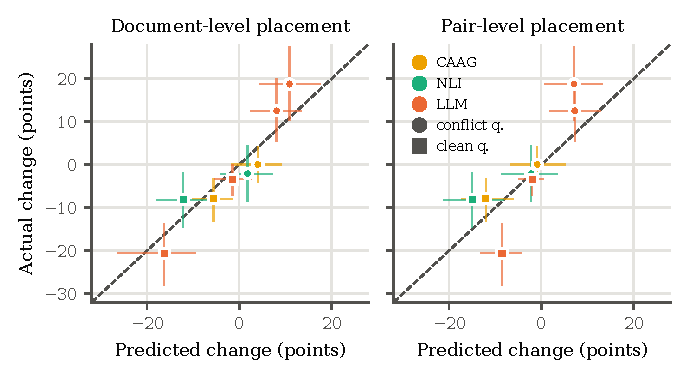
\includegraphics[width=\columnwidth]{generated/fig_placement.pdf}
\caption{Effect of real detectors predicted from the synthetic grid (x, with the 95\% bootstrap prediction interval)
against the measured effect (y, with its 95\% CI), for conflict ($\bullet$) and clean ($\blacksquare$) questions.
Left: detectors located by their document-level behaviour; right: by pair precision, recall and direction accuracy.}
\label{fig:placement}
\end{figure}

\paragraph{The heuristic detector.}
CAAG, the detector we set out to study, scores a pair only if its MiniLM \citep{reimers2019sbert} cosine similarity reaches $\theta_s=0.65$. Its score
is the sum of a negation and contrast asymmetry term, a named-entity mismatch term (differing dates, numbers, money or
percentages) and a temporal-marker term, multiplied by the similarity. A pair is flagged if the score reaches
$\theta_c=0.35$. Its per-pair flag rate on the confirmatory split ($6.22\%$) sets the random detector's rate.
As a neutral flag, CAAG did not beat random flags of the same volume, and
as a removal rule it only deleted correct passages (\dCaagRemClean\ points on clean questions, \dCaagRemConf\ on
conflict ones). Its false flags fall mostly on pairs that should both be reported: 134 of its 221 false flags on the
hold-out are same-name ambiguity pairs, flagged by its entity-mismatch signal for mentioning different dates or
numbers. We read this as a warning about lexical contradiction cues in general \citep{gururangan2018annotation},
not about a particular threshold. Retuning shows why F1 misleads: over a 121-setting sweep, CAAG's
best pair F1 is \caagBestFOne, above NLI's, at $\theta_s=\caagBestThS$ and $\theta_c=\caagBestThC$, but by flagging \caagBestRate\% of all pairs and \caagBestCleanFpr\% of clean questions, which our grid predicts
would be harmful under removal (Appendix~\ref{app:grid}).

\paragraph{Original CAAG format.}
Rendering CAAG's flags in its original format, with typed lines and confidence scores (``factual conflict (confidence:
0.41)''), changes accuracy by \origCaagAll\ points overall (\origCaagConf\ on conflict questions, \origCaagClean\ on
clean ones). It is no different from the uniform format.

\paragraph{Pilot study (exploratory).}
On the 200-question pilot split, scored with the bidirectional metric, the same pattern appeared before any
confirmatory run. Oracle neutral flags changed conflict-question accuracy by $-$10.5 points, directional flags by
$+$11.8, and removing the suspect by $+$28.4. The pilots also showed that the original \textsc{remove} strategy,
which deletes an arbitrary side of each pair, removes correct documents. The pilots led us to add directional formats,
synthetic direction accuracy and document-level placement. All pilot runs are released.

\paragraph{Phase-0 audit of CAAG on NarrativeQA.}
CAAG was designed for long-document QA. On 100 NarrativeQA \citep{kocisky2018narrativeqa} questions from 50 stories
(BM25 top-10 chunks from a single coherent story), it flags at least one pair in 54\% of questions, 166 pairs in all.
A single story rarely contradicts itself, so most of these flags are likely false. The flagged pairs are released for annotation.

\section{Further Results}
\label{app:more}

\begin{figure}[t]
\centering
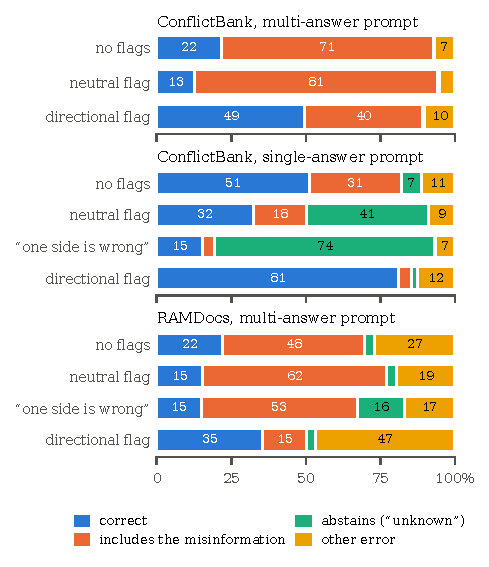
\includegraphics[width=\columnwidth]{generated/fig_answers.pdf}
\caption{What a flag does to answers on conflict questions (gpt-4o-mini, oracle pairs; share of answers, \%). The
answer policy decides how a neutral flag fails: a model told to give every valid answer adds the misinformation, and
one told there is one answer abstains. Only the directional flag raises the share of correct answers. Categories are exclusive and an answer the primary metric scores correct counts as correct, so the misinformation share can be slightly lower than in Table~\ref{tab:risk}, which counts every answer containing a wrong answer under the bidirectional matcher.}
\label{fig:answers}
\end{figure}
\begin{table*}[t]
\centering\small
\setlength{\tabcolsep}{4pt}
\begin{tabular}{lrrrrrrrr}
\toprule
& \multicolumn{3}{c}{RAMDocs, gpt-4o-mini} & RAMDocs, gpt-4.1 & \multicolumn{3}{c}{ConflictBank, gpt-4o-mini} & \\
\cmidrule(lr){2-4}\cmidrule(lr){5-5}\cmidrule(lr){6-8}
Method & Lab. & Conflict & Clean & Lab. & All & Conflict & Clean & Calls \\
\midrule
No flags (plain), accuracy & 31.3 & 22.1 & 41.5 & 32.8 & 38.4 & 21.6 & 89.0 & 1 \\
\midrule
Instruction (v2) only & $+$2.3 & $+$5.3 & $-$1.1 & -- & $+$4.0 & $+$5.9 & $-$1.7 & 1 \\
Oracle, flag + instr. & $-$1.8 & $-$2.4 & $-$1.1 & $+$1.5 & $+$0.7 & $+$1.6 & $-$1.7 & 1 \\
Oracle, dir.\ flag + instr. & $+$6.4 & $+$13.2 & $-$1.1 & \textbf{$+$14.7} & \textbf{$+$47.4} & \textbf{$+$63.8} & $-$1.7 & 1 \\
\midrule
MADAM-RAG & $+$5.7 & $+$3.6 & $+$7.9 & -- & -- & -- & -- & 9$\times$tok. \\
Astute RAG & \textbf{$-$15.6} & $-$8.4 & \textbf{$-$23.5} & -- & \textbf{$+$18.2} & \textbf{$+$27.4} & $-$9.7 & 2 \\
Astute RAG (multi) & $-$5.9 & $-$1.2 & $-$11.1 & $+$2.3 & -- & -- & -- & 2 \\
TrustRAG & \textbf{$-$17.5} & $-$11.3 & \textbf{$-$24.3} & -- & \textbf{$+$13.9} & \textbf{$+$19.9} & $-$4.0 & 3 \\
TrustRAG (multi) & \textbf{$-$18.1} & $-$12.2 & \textbf{$-$24.6} & $-$10.9 & -- & -- & -- & 3 \\
\midrule
LLM detector, flag + instr. & $-$2.0 & $-$2.2 & $-$1.9 & -- & -- & -- & -- & 1 \\
LLM detector, dir.\ flag + instr. & $-$3.5 & $+$8.4 & \textbf{$-$16.7} & -- & -- & -- & -- & 1 \\
LLM detector, dir.\ flag & $+$4.9 & $+$12.5 & $-$3.4 & \textbf{$+$8.7} & \textbf{$+$14.8} & \textbf{$+$20.0} & $-$1.0 & 1 \\
LLM detector, remove suspect & 0.0 & \textbf{$+$18.7} & \textbf{$-$20.6} & -- & \textbf{$+$27.4} & \textbf{$+$38.8} & $-$6.7 & 1 \\
\bottomrule
\end{tabular}
\caption{Resolution instructions and published baselines. First row: accuracy (\%, one-way strict) with no flags; other rows:
paired difference from it in points. \emph{Lab.}: the labelled RAMDocs questions; ConflictBank questions are all
labelled. RAMDocs gpt-4o-mini and ConflictBank: 3 seeds; RAMDocs gpt-4.1: seed 0. \emph{instr.}: the v2 reliability
instruction. \emph{(multi)}: the baseline's final step asks for every valid answer, which RAMDocs needs (every
ConflictBank question has one answer). Calls: generator calls per question (LLM-detector rows add one detector call).
\textbf{Bold}: significant under the paper's single scheme (Section~\ref{sec:setup}).}
\label{tab:baselines}
\end{table*}

\begin{table}[t]
\centering\footnotesize
\setlength{\tabcolsep}{3pt}
\begin{tabular}{llrrrr}
\toprule
Detector & Generator & Dir.\ acc. & Gen.\ acc. & Gap & Gain \\
\midrule
gpt-6.1-terra & gpt-6.1-terra & 29.7 & 73.0 & $-$43.3 & $+$2.7 \\
gpt-6.1-terra & Claude Haiku 5.5 & 29.7 & 66.8 & $-$37.1 & \textbf{$+$4.1} \\
gpt-6.1-terra & gpt-4.1 & 29.7 & 64.7 & $-$35.0 & \textbf{$+$5.0} \\
gpt-6-luna & gpt-6.1-terra & 45.7 & 73.0 & $-$27.3 & $+$2.7 \\
gpt-6.1-terra & gpt-6-luna & 29.7 & 53.6 & $-$23.9 & \textbf{$+$7.3} \\
gpt-6-luna & Claude Haiku 5.5 & 45.7 & 66.8 & $-$21.1 & \textbf{$+$5.0} \\
gpt-6.1-terra & gpt-4o-mini & 31.3 & 51.1 & $-$19.8 & \textbf{$+$9.6} \\
gpt-6.1-terra & Qwen2.5-7B & 31.0 & 50.3 & $-$19.3 & \textbf{$+$8.0} \\
gpt-6-luna & gpt-4.1 & 45.7 & 64.7 & $-$19.0 & \textbf{$+$6.3} \\
gpt-6-luna & gpt-6-luna & 45.7 & 53.6 & $-$7.9 & \textbf{$+$11.1} \\
gpt-4o-mini & gpt-6.1-terra & 67.0 & 73.0 & $-$6.0 & \textbf{$-$11.7} \\
gpt-6-luna & gpt-4o-mini & 45.7 & 51.1 & $-$5.4 & \textbf{$+$13.7} \\
Claude Haiku 5.5 & Claude Haiku 5.5 & 61.7 & 66.8 & $-$5.1 & \textbf{$+$5.7} \\
gpt-6-luna & Qwen2.5-7B & 48.0 & 50.3 & $-$2.3 & \textbf{$+$12.0} \\
Claude Sonnet 5.5 & Claude Haiku 5.5 & 65.0 & 66.8 & $-$1.8 & \textbf{$+$8.2} \\
gpt-4o-mini & Claude Haiku 5.5 & 67.0 & 66.8 & $+$0.2 & $-$4.1 \\
gpt-4o-mini & gpt-4.1 & 67.0 & 64.7 & $+$2.3 & $-$2.3 \\
gpt-4.1 & gpt-6.1-terra & 79.0 & 73.0 & $+$6.0 & \textbf{$+$7.3} \\
Claude Haiku 5.5 & gpt-6-luna & 61.7 & 53.6 & $+$8.1 & \textbf{$+$14.3} \\
Claude Haiku 5.5 & gpt-4o-mini & 61.7 & 51.1 & $+$10.6 & \textbf{$+$13.0} \\
Claude Sonnet 5.5 & gpt-6-luna & 65.0 & 53.6 & $+$11.4 & \textbf{$+$18.1} \\
gpt-4.1 & Claude Haiku 5.5 & 79.0 & 66.8 & $+$12.2 & \textbf{$+$11.0} \\
gpt-4o-mini & gpt-6-luna & 67.0 & 53.6 & $+$13.4 & \textbf{$+$8.6} \\
Claude Sonnet 5.5 & gpt-4o-mini & 65.0 & 51.1 & $+$13.9 & \textbf{$+$15.9} \\
gpt-4.1 & gpt-4.1 & 79.0 & 64.7 & $+$14.3 & \textbf{$+$11.7} \\
gpt-4o-mini & gpt-4o-mini & 67.0 & 51.1 & $+$15.9 & \textbf{$+$8.4} \\
gpt-4o-mini & Qwen2.5-7B & 67.0 & 50.3 & $+$16.7 & \textbf{$+$7.3} \\
gpt-4.1 & gpt-6-luna & 79.0 & 53.6 & $+$25.4 & \textbf{$+$21.3} \\
gpt-4.1 & gpt-4o-mini & 79.0 & 51.1 & $+$27.9 & \textbf{$+$18.6} \\
gpt-4.1 & Qwen2.5-7B & 79.3 & 50.3 & $+$29.0 & \textbf{$+$16.0} \\
\bottomrule
\end{tabular}
\caption{Every detector--generator cell of H24 (ConflictBank, one-answer prompt, 300 conflict questions; \%).
\emph{Dir.\ acc.}: share of questions on which the detector flags the true contradiction and names its misinformation
passage; \emph{Gen.\ acc.}: the generator's accuracy with no flags; \emph{Gain}: the LLM directional flag's change in
points. Figure~\ref{fig:reliability} plots the same cells.}
\label{tab:cells}
\end{table}

\begin{table}[t]
\centering\footnotesize
\setlength{\tabcolsep}{3pt}
\resizebox{\columnwidth}{!}{%
\begin{tabular}{lr}
\toprule
\multicolumn{2}{l}{\emph{Cell level (30 cells): accuracy with the flag, $A$}} \\
$A \sim D + G$: coefficient of $D$ & 0.09 [0.03, 0.16] \\
\quad coefficient of $G$ & 0.46 [0.36, 0.55] \\
$A \sim D$ + generator FE: coefficient of $D$ & 0.09 [0.02, 0.15] \\
\quad exact permutation of $D$ across detectors & $p=0.29$ \\
\midrule
\multicolumn{2}{l}{\emph{Leave one detector out: $R^2$ for the gain}} \\
$G$ only & 0.17 \\
$D+G$ & $-$0.07 \\
gap $D-G$ (registered) & $-$0.21 \\
mechanism score & 0.62 \\
\midrule
\multicolumn{2}{l}{\emph{Question level (9000 cell-questions), points}} \\
detector right on $q$ & $+$34.5 [$+$32.8, $+$36.1] \\
detector marks a correct passage & $-$31.6 [$-$33.9, $-$29.4] \\
generator right on its own & $+$37.9 [$+$36.3, $+$39.5] \\
\midrule
\multicolumn{2}{l}{\emph{Calibration: gain $\sim$ score}} \\
slope & 0.64 [0.54, 0.74] \\
\bottomrule
\end{tabular}}

\vspace{4pt}
\begin{tabular}{lrr}
\toprule
Generator & Follows a needed & Follows a wrong- \\
& right flag & side flag \\
\midrule
Qwen2.5-7B & 61 (327) & 77 (71) \\
Claude Haiku & 57 (189) & 83 (71) \\
gpt-4.1 & 69 (171) & 83 (60) \\
gpt-4o-mini & 66 (446) & 76 (75) \\
gpt-6-luna & 75 (281) & 84 (58) \\
gpt-6.1-terra & 68 (154) & 88 (97) \\
\bottomrule
\end{tabular}
\caption{H24 without the shared $-G$ term (\S15.4, re-analysis of existing cells). $D$: the detector's direction
accuracy; $G$: the generator's no-flag accuracy. CIs: 2,000 question resamples, shared across cells. The question-level
model is a linear probability model with detector and generator fixed effects and a random intercept per question.
Lower table: share of questions the generator gets right when the detector is right and the generator alone is wrong
in every seed, and share it gets wrong when the detector marks a correct passage and the generator alone is right in
every seed (count of cell-questions in brackets).}
\label{tab:h24redo}
\end{table}

\begin{table*}[t]
\centering\footnotesize
\setlength{\tabcolsep}{4pt}
\begin{tabular}{lrlr}
\toprule
Setting & Neutral flag & Setting & Neutral flag \\
\midrule
CB forced, gpt-6.1-terra & $-$0.3 & RAMDocs, Claude Haiku & $+$1.2 \\
CB forced, gpt-4o-mini & $-$0.2 & CB one-answer, gpt-4o-mini & $-$18.7 \\
CB forced, gpt-6-luna & $+$1.6 & CB one-answer, gpt-6-luna & $-$9.4 \\
CB forced, Claude Haiku & $+$3.9 & CB one-answer, gpt-4.1 & $-$8.0 \\
CB minimal, gpt-4o-mini & $-$18.1 & CB majority, gpt-6.1-terra & $-$3.7 \\
RAMDocs, gpt-4.1 (minimal) & $-$11.0 & CB one-answer, Qwen2.5-7B & $-$3.3 \\
RAMDocs, Qwen2.5-7B (minimal) & $-$5.8 & CB one-answer, gpt-6.1-terra & $-$2.3 \\
RAMDocs, gpt-4o-mini (minimal) & $-$5.3 & RAGuard, gpt-6-luna & 0.0 \\
CB multi-answer, gpt-4o-mini & $-$8.8 & RAGuard, Claude Haiku & $+$0.3 \\
RAMDocs, gpt-4.1 (multi-answer) & $-$8.6 & CB one-answer, Claude Haiku & $+$0.7 \\
CB multi-answer, Qwen2.5-7B & $-$8.3 & CB majority, gpt-4o-mini & $+$1.1 \\
RAMDocs, gpt-4o-mini (multi-answer) & $-$6.7 & RAGuard, gpt-6.1-terra & $+$2.4 \\
CB multi-answer, gpt-4.1 & $-$6.3 & CB one-answer, Claude Sonnet & $+$3.0 \\
RAMDocs, Qwen2.5-7B (multi-answer) & $-$5.8 & RAGuard, gpt-4o-mini & $+$3.2 \\
RAMDocs, gpt-6-luna & $-$3.1 & CB majority, Claude Haiku & $+$4.3 \\
RAMDocs, gpt-6.1-terra & $-$0.7 & RAGuard, Claude Sonnet & $+$4.4 \\
RAMDocs, Claude Sonnet & 0.0 & CB majority, gpt-6-luna & $+$6.6 \\
\midrule
\multicolumn{4}{l}{\emph{Multilevel model (random effects for generator, benchmark and setting; REML)}} \\
\multicolumn{2}{l}{pooled, all settings} & \multicolumn{2}{l}{\neuMlMu\ \neuMlCI; prediction interval \neuMlPI} \\
\multicolumn{2}{l}{pooled, multi-answer prompt (10 settings)} & \multicolumn{2}{l}{$-$3.8 [$-$6.5, $-$1.0]} \\
\multicolumn{2}{l}{pooled, minimal prompt (4 settings)} & \multicolumn{2}{l}{$-$12.1 [$-$23.6, $-$0.7]} \\
\multicolumn{2}{l}{pooled, one answer prompt (16 settings)} & \multicolumn{2}{l}{$-$0.5 [$-$5.5, $+$4.5]} \\
\multicolumn{2}{l}{pooled, forced prompt (4 settings)} & \multicolumn{2}{l}{$+$1.5 [$-$1.3, $+$4.3]} \\
\midrule
\multicolumn{4}{l}{\emph{Meta-regression (same model)}} \\
\multicolumn{2}{l}{intercept (OpenAI, one answer, generated)} & \multicolumn{2}{l}{$-$2.8 [$-$8.1, $+$2.6]} \\
\multicolumn{2}{l}{several answers allowed} & \multicolumn{2}{l}{$-$3.5 [$-$8.2, $+$1.2]} \\
\multicolumn{2}{l}{forced (no unknown)} & \multicolumn{2}{l}{$+$6.4 [$+$1.6, $+$11.2]} \\
\multicolumn{2}{l}{Anthropic} & \multicolumn{2}{l}{$+$5.2 [$+$1.7, $+$8.7]} \\
\multicolumn{2}{l}{Qwen} & \multicolumn{2}{l}{$+$1.0 [$-$4.0, $+$6.0]} \\
\multicolumn{2}{l}{natural misinformation (RAGuard)} & \multicolumn{2}{l}{$+$2.7 [$-$7.0, $+$12.3]} \\
\bottomrule
\end{tabular}
\caption{The 34 settings in which the oracle neutral flag was run (conflict questions, change in
points), grouped by answer policy. The pooled estimate was registered as exploratory (\S13.4) and the multilevel model,
the policy split and the moderators in \S16.4; they use data already seen. The prediction interval describes this
design space (our generators, benchmarks and prompts), not deployments in general. \emph{Natural misinformation} is
RAGuard only; RAMDocs' misinformation is synthetic.}
\label{tab:pooled}
\end{table*}

\begin{table*}[t]
\centering\footnotesize
\setlength{\tabcolsep}{3.5pt}
\resizebox{\textwidth}{!}{%
\begin{tabular}{lrrrrrrrrr}
\toprule
& \multicolumn{4}{c}{Neutral flag, utility change at misinformation cost $c$} & Dir.\ flag & \multicolumn{4}{c}{Neutral flag: plain answer $\to$ flagged answer (null)} \\
\cmidrule(lr){2-5}\cmidrule(lr){6-6}\cmidrule(lr){7-10}
Setting & $c=0$ & $c=1$ & $c=2$ & $c=4$ & $c=2$ & mis.$\to$abst. & mis.$\to$corr. & corr.$\to$abst. & corr.$\to$mis. \\
\midrule
RAMDocs, gpt-4o-mini (multi-answer) & \textbf{$-$6.7} & \textbf{$-$20.9} & \textbf{$-$35.0} & \textbf{$-$63.3} & \textbf{$+$79.1} & 1 (0) & 2 (2) & 0 (0) & 29 (3) \\
RAMDocs, gpt-6-luna & \textbf{$-$3.1} & $-$7.7 & $-$12.2 & $-$21.3 & \textbf{$+$160.9} & 0 (0) & 1 (3) & 0 (0) & 22 (16) \\
RAMDocs, Claude Haiku & $+$1.2 & $+$9.1 & \textbf{$+$17.0} & \textbf{$+$32.9} & \textbf{$+$125.2} & 0 (0) & 9 (4) & 0 (0) & 5 (9) \\
CB multi-answer, gpt-4o-mini & \textbf{$-$8.8} & \textbf{$-$19.2} & \textbf{$-$29.7} & \textbf{$-$50.6} & \textbf{$+$91.0} & 0 (0) & 4 (3) & 1 (0) & 55 (9) \\
CB one-answer, gpt-4o-mini & \textbf{$-$18.7} & $-$5.3 & $+$8.0 & \textbf{$+$34.7} & \textbf{$+$83.7} & 45 (2) & 7 (3) & 37 (1) & 5 (2) \\
CB one-answer, gpt-6-luna & \textbf{$-$9.4} & $-$2.6 & $+$4.3 & $+$18.1 & \textbf{$+$85.1} & 27 (10) & 12 (13) & 20 (6) & 5 (6) \\
CB one-answer, gpt-6.1-terra & $-$2.3 & 0.0 & $+$2.3 & $+$7.0 & \textbf{$+$51.7} & 2 (--) & 26 (--) & 4 (--) & 5 (--) \\
CB one-answer, Claude Haiku & $+$0.7 & $+$0.6 & $+$0.4 & $+$0.2 & \textbf{$+$66.9} & 0 (0) & 25 (16) & 0 (0) & 8 (5) \\
CB one-answer, Claude Sonnet & $+$3.0 & $+$6.7 & $+$10.3 & $+$17.7 & \textbf{$+$45.7} & 2 (--) & 34 (--) & 0 (--) & 3 (--) \\
CB forced, gpt-4o-mini & $-$0.2 & $-$0.6 & $-$0.9 & $-$1.6 & \textbf{$+$74.0} & 1 (0) & 19 (4) & 0 (0) & 11 (2) \\
CB majority, gpt-4o-mini & $+$1.1 & \textbf{$+$24.6} & \textbf{$+$48.0} & \textbf{$+$94.9} & \textbf{$+$118.2} & 26 (1) & 11 (2) & 22 (1) & 8 (5) \\
RAGuard, gpt-4o-mini & $+$3.2 & $+$6.6 & $+$10.0 & $+$16.8 & \textbf{$+$34.6} & 12 (3) & 7 (3) & 8 (6) & 4 (2) \\
RAGuard, gpt-6-luna & 0.0 & $-$1.1 & $-$2.3 & $-$4.5 & \textbf{$+$29.3} & 10 (9) & 6 (9) & 8 (9) & 7 (8) \\
RAGuard, Claude Haiku & $+$0.3 & $-$1.8 & $-$4.0 & $-$8.3 & \textbf{$+$26.5} & 7 (6) & 4 (4) & 11 (9) & 6 (3) \\
\bottomrule
\end{tabular}}
\caption{Abstention-aware view of the oracle flags (conflict questions; \S15.4 and \S16.4, re-analyses of data already
seen). Utility per answer: $+1$ correct, $-c$ if it contains the misinformation, 0 for abstaining or any other wrong
answer; $c=0$ is strict accuracy. Bold: significant in one Holm family per $c$ over all \nUtilSixSettings\ settings of
Table~\ref{tab:pooled} (a selection is shown). Right: of the question--seed pairs whose plain answer contained the
misinformation (or was correct), the share whose flagged answer abstained, was correct or contained the misinformation;
in brackets the same share between two plain runs with different seeds, the churn with no flag.}
\label{tab:utility}
\end{table*}


\subsection{Where the directional flag fails (exploratory)}
\label{app:single}
After seeing the minimal-skeleton run, we split conflict questions by number of gold answers. \nConfMulti\ of
\the\numexpr\nConfMulti+\nConfSingle\relax\ have several (same-name ambiguity \emph{and} misinformation), and a strict
answer must list them all. On the \nConfSingle\ single-answer conflict questions, the directional flag's estimate
is positive in every setting, from \yQwenSingleOracleDir\ points (Qwen) to \yMiniSingleOracleDir\ (gpt-4o-mini), both
with the default skeleton. On multi-answer questions it changes little except with gpt-4.1 (gpt-4o-mini
\yMiniMultiOracleDir, and \yMiniMinMultiOracleDir\ with the minimal skeleton; gpt-4.1 \yFourMultiOracleDir). One untested
reading is that a warning about one passage makes the smaller models more conservative about legitimate
alternative answers too. Removal, which needs no warning to be acted on, gains in both groups.

\subsection{Real detectors}
CAAG flags \cleanFprCaag\% of clean questions. Its neutral flags do not beat random flags at the same rate (H5;
\dCaagFlagAll\ vs.\ \dRandFlagAll\ points overall). The 90\% CI of the difference, [\tostLo, \tostHi], rules out a
gain above \tostHi\ points but does not establish equivalence within $\pm$\tostMargin\ points (TOST). The
addendum registered the LLM detector's directional-versus-neutral comparison as exploratory.
Under the bidirectional metric, the LLM detector's directional flag costs clean questions \arLlmDirClean\ points. With
gpt-4.1 generating, its gain over all 300 questions (\gptLlmDirAll) is significant after Holm, but the 35
unlabelled questions contribute disproportionately (they gain \agptexclLlmDir\ points). On labelled
questions it is \gptlabLlmDir\ \gptlabLlmDirCI. On ConflictBank the NLI cross-encoder flags no pair:
the benchmark's passages are long, LLM-written and agree on everything but the one fact, and the truncated pair rarely
contains it.

\paragraph{Stronger models abstain in the single call.} Asked to name suspect passages before answering, the reasoning
models and Claude Haiku distrust most of ConflictBank's generated passages and abstain, losing up to
\azSgTerraSelfIdentifyClean\ points on clean questions (Table~\ref{tab:baselines}).

\paragraph{Reasoning models on RAMDocs.} Without flags, gpt-6-luna and gpt-6.1-terra are
strictly correct on few RAMDocs conflict questions because the default prompt asks for every valid answer. They give
\mixRdLunaNAnswers\ and \mixRdTerraNAnswers\ answers on average and recover \mixRdLunaRecall\% and
\mixRdTerraRecall\% of gold answers, but \mixRdLunaMisinfo\% and \mixRdTerraMisinfo\% of their answers include
the misinformation.

\paragraph{Detector parsing.} The LLM detectors' JSON failed to parse on \parseFailTotal\ of \parseFailN\ ConflictBank
questions (a Claude Sonnet output), counted as flagging nothing.

\subsection{A detector from another family}
Replacing the gpt-4o-mini detector with Qwen2.5-7B (gpt-4o-mini still generates) gives a much less selective
detector: it flags \qdetFpr\% of clean RAMDocs questions, but its direction accuracy is \qdetDir\%. Its directional
flag gains \zQDetLlmDirFlagDirectionalConflict\ points on conflict questions and \zQDetLlmDirFlagDirectionalClean\ on
clean ones, and its neutral flag \zQDetLlmDirFlagConflict. Removal again trades a conflict-question gain
(\zQDetLlmDirRemoveSuspectConflict) for a clean-question loss (\zQDetLlmDirRemoveSuspectClean). The conclusions do
not depend on the detector's family.

\subsection{CONFLICTS}
On the 237 automatically scorable CONFLICTS questions (exploratory, 3 seeds; most have no conflict), no condition
moves accuracy significantly (Table~\ref{tab:conflicts}).

\section{Semantic Re-score, Label Audits and Selection}
\label{app:semantic}
\begin{table*}[t]
\centering\scriptsize
\setlength{\tabcolsep}{4pt}
\begin{tabular}{llrrr}
\toprule
Setting & Contrast & Matcher (points) & Judge (points) & Judge $-$ matcher \\
\midrule
RAMDocs, gpt-4o-mini & neutral flag vs plain & $-$4.2 [$-$9.2, 0.0] & $-$2.5 [$-$9.2, $+$4.2] & $+$1.7 [$-$3.3, $+$6.7] \\
ConflictBank, gpt-4o-mini & neutral flag vs plain & $-$20.0 [$-$27.5, $-$12.5] & $-$21.7 [$-$29.2, $-$14.2] & $-$1.7 [$-$4.2, 0.0] \\
ConflictBank, Claude Haiku & neutral flag vs plain & $+$3.3 [$-$3.3, $+$10.0] & $+$6.7 [$+$0.8, $+$13.3] & $+$3.3 [0.0, $+$7.5] \\
RAMDocs, gpt-4o-mini & oracle directional flag vs answer key & $-$0.8 [$-$5.8, $+$4.2] & $+$0.8 [$-$8.3, $+$10.0] & $+$1.7 [$-$6.7, $+$10.0] \\
ConflictBank, gpt-4o-mini & oracle directional flag vs answer key & $+$10.8 [$+$4.2, $+$17.5] & $+$12.5 [$+$6.7, $+$19.2] & $+$1.7 [$-$1.7, $+$5.0] \\
ConflictBank, gpt-6-luna & oracle directional flag vs answer key & $-$1.7 [$-$5.8, $+$2.5] & 0.0 [$-$3.3, $+$3.3] & $+$1.7 [$-$1.7, $+$5.0] \\
ConflictBank, gpt-4o-mini & LLM directional flag vs verdict key & $+$3.3 [$-$2.5, $+$9.2] & $+$6.7 [$+$0.8, $+$12.5] & $+$3.3 [0.0, $+$7.5] \\
ConflictBank, gpt-6-luna & LLM directional flag vs verdict key & $-$0.8 [$-$3.3, $+$1.7] & 0.0 [$-$2.5, $+$2.5] & $+$0.8 [$-$1.7, $+$4.2] \\
ConflictBank, gpt-4o-mini & randomised directional flag vs plain & $+$4.2 [$-$5.8, $+$15.0] & $+$6.7 [$-$3.3, $+$16.7] & $+$2.5 [0.0, $+$5.8] \\
ConflictBank, Claude Haiku & randomised directional flag vs plain & $-$7.5 [$-$18.3, $+$3.3] & $-$6.7 [$-$17.5, $+$4.2] & $+$0.8 [$-$1.7, $+$3.3] \\
\bottomrule
\end{tabular}

\vspace{4pt}
\begin{tabular}{lrrrrr}
\toprule
Condition & Outputs & Matcher (\%) & Judge (\%) & Judge only (\%) & Matcher only (\%) \\
\midrule
answer key & 360 & 67.8 & 77.8 & 10.3 & 0.3 \\
directional flag (LLM) & 240 & 59.6 & 62.5 & 3.8 & 0.8 \\
directional flag (oracle) & 360 & 70.6 & 82.2 & 11.7 & 0.0 \\
neutral flag (oracle) & 360 & 36.9 & 43.3 & 6.9 & 0.6 \\
no flag & 600 & 48.8 & 53.3 & 5.2 & 0.7 \\
randomised direction (H31) & 240 & 54.6 & 59.6 & 5.0 & 0.0 \\
verdict key (LLM) & 240 & 58.3 & 59.2 & 2.1 & 1.2 \\
\bottomrule
\end{tabular}
\caption{Semantic re-score (\S17.3; exploratory). An outside-family judge (gemini-3.5-flash-lite, temperature 0) reads
the question, the reference and known wrong answers and the response, and classifies the final answer; judge-strict
means it gives the reference answer, asserts no wrong one and does not abstain. Top: each contrast on the same
120 conflict questions (seed 0) under the matcher and the judge, and their difference, with question-bootstrap
95\% CIs. Bottom: per condition, the share scored correct by each and the shares where only one does. The judge is
an LLM given the answer keys: it checks the matcher's semantics, not the benchmark labels.}
\label{tab:semantic}
\end{table*}

\paragraph{An outside-family judge changes no contrast's sign (\S17.3).} To
check whether the primary metric's string-matching errors differ by condition, an LLM from outside our generators' families re-scored both
arms of \semK\ contrasts on the same \semNq\ conflict questions each (gemini-3.5-flash-lite; Table~\ref{tab:semantic}).
\S17.3 named Gemini 2.5 Flash, which was closed to new users. Judge and matcher agree on \semAgree\% of \semN\ outputs. Almost all
disagreements are answers the judge accepts and the matcher rejects (aliases, paraphrases, partial forms) and
depend on condition: \semJudgeOnlyKey\% of answer-key outputs and \semJudgeOnlyDir\% of oracle-directional ones,
against \semJudgeOnlyPlain\% without a flag. The failure of most concern, a final answer such as
``$Y$, not $X$'' counted as asserting the wrong answer $X$, occurs in \semRejected\% of outputs. Because
both arms of each contrast gain, the judge moves every contrast by \semDidMin\ to \semDidMax\ points. No conclusion
changes sign; the matcher-scored differences are slightly conservative. With \semNq\ questions per contrast these
intervals are too wide to confirm the $\pm$3-point equivalence claims, which therefore rest on the matcher. Given
the gold and wrong answers, the judge tests the scorer, not the benchmark labels. A blinded, paired human-audit sheet of
150 of these pairs and 50 RAGuard post pairs is released unlabelled (\texttt{runs/labelling/audit8\_*}).

\paragraph{The WikiContradict harm holds under its original rubric.} The original rubric counts an answer correct when it gives
both answers, acknowledges that they conflict and does not prefer one without support
\citep[\S3.4]{hou2024wikicontradict}. Under it, the LLM directional flag changes the share of correct answers
by \wikiOrigMiniEff\ points for gpt-4o-mini (\wikiOrigMiniPlain\% to \wikiOrigMiniDir\%), \wikiOrigLunaEff\ for
gpt-6-luna and \wikiOrigHaikuEff\ for Claude Haiku (seed 0, all 253 questions), so the H28 harm holds. For gpt-4o-mini the flag raises the share that merely mentions both answers (\wikiBothMiniEff) while
lowering the share that acknowledges the conflict without an unsupported preference.

\paragraph{RAGuard pairs rarely contradict.} RAGuard labels a post supporting or misleading by whether GPT-4 judged the claim correctly
with it in context, so its ``contradiction pairs'' transfer behavioural labels. Of \rgAudN\ sampled
supporting~$\times$~misleading pairs, the judge finds the two posts cannot both be right about the claim in
\rgAudContradict\%. It finds the misleading post false about the claim in \rgAudBFalse\% (unclear in
\rgAudBUnclear\%) and the supporting post consistent with the verdict in \rgAudASupports\%. All three hold for
\rgAudVerified\%. Most pairs discuss the claim from different angles rather than assert opposite
facts. RAGuard's oracle-flag rows therefore test what a generator does with these labels, not with verified
contradictions; we draw no factual-oracle conclusion from them. This audit uses one LLM judge; the released
human sheet covers 50 of these pairs.

\begin{table*}[t]
\centering\scriptsize
\setlength{\tabcolsep}{3pt}
\begin{tabular}{llrrrrrrrrrrrr}
\toprule
& & & & \multicolumn{3}{c}{Flag names the false side} & \multicolumn{3}{c}{Flag marks a correct passage} & Rest & \multicolumn{3}{c}{Gain (points)} \\
\cmidrule(lr){5-7}\cmidrule(lr){8-10}\cmidrule(lr){12-14}
Generator & Detector & Prec. & Rec. & Share & Acc. & Gain & Share & Acc. & Gain & contrib. & Marginal & Question & Observed \\
\midrule
gpt-4o-mini & Claude Haiku & 78 & 79 & 62 & 58 & $+$28.8 & 11 & 42 & $-$30.4 & $-$1.3 & $+$16.1 & $+$12.3 & $+$13.0 \\
gpt-4o-mini & Claude Sonnet & 78 & 84 & 65 & 51 & $+$32.8 & 10 & 40 & $-$20.7 & $-$3.4 & $+$15.8 & $+$16.1 & $+$15.9 \\
gpt-4o-mini & gpt-4.1 & 82 & 97 & 79 & 55 & $+$28.6 & 8 & 25 & $-$22.2 & $-$2.2 & $+$18.3 & $+$19.2 & $+$18.6 \\
gpt-4o-mini & gpt-4o-mini & 69 & 97 & 67 & 60 & $+$23.1 & 30 & 30 & $-$23.1 & 0.0 & $+$10.5 & $+$10.4 & $+$8.4 \\
gpt-4o-mini & gpt-6-luna & 82 & 56 & 46 & 50 & $+$36.7 & 7 & 57 & $-$46.7 & 0.0 & $+$18.5 & $+$11.0 & $+$13.7 \\
gpt-4o-mini & gpt-6.1-terra & 83 & 38 & 31 & 51 & $+$36.9 & 4 & 61 & $-$36.1 & $-$0.6 & $+$19.2 & $+$7.4 & $+$9.6 \\
gpt-6-luna & Claude Haiku & 78 & 79 & 62 & 61 & $+$31.5 & 11 & 45 & $-$34.3 & $-$1.2 & $+$16.3 & $+$13.5 & $+$14.3 \\
gpt-6-luna & Claude Sonnet & 78 & 84 & 65 & 59 & $+$34.5 & 10 & 41 & $-$35.6 & $-$0.9 & $+$16.0 & $+$16.2 & $+$18.1 \\
gpt-6-luna & gpt-4.1 & 82 & 97 & 79 & 60 & $+$31.1 & 8 & 21 & $-$20.8 & $-$1.6 & $+$19.2 & $+$21.6 & $+$21.3 \\
gpt-6-luna & gpt-4o-mini & 69 & 97 & 67 & 63 & $+$27.0 & 30 & 33 & $-$31.5 & 0.0 & $+$9.1 & $+$10.0 & $+$8.6 \\
gpt-6-luna & gpt-6-luna & 82 & 56 & 46 & 64 & $+$29.2 & 7 & 40 & $-$35.0 & $+$0.1 & $+$19.4 & $+$9.8 & $+$11.1 \\
gpt-6-luna & gpt-6.1-terra & 82 & 36 & 30 & 66 & $+$30.3 & 4 & 56 & $-$38.5 & 0.0 & $+$19.7 & $+$5.4 & $+$7.3 \\
Claude Haiku & Claude Haiku & 78 & 79 & 62 & 79 & $+$14.8 & 11 & 28 & $-$22.5 & $-$0.9 & $+$8.0 & $+$6.1 & $+$5.7 \\
Claude Haiku & Claude Sonnet & 78 & 84 & 65 & 74 & $+$18.1 & 10 & 53 & $-$37.9 & $+$0.1 & $+$7.8 & $+$7.3 & $+$8.2 \\
Claude Haiku & gpt-4.1 & 82 & 97 & 79 & 73 & $+$18.0 & 8 & 17 & $-$16.7 & $-$1.9 & $+$10.7 & $+$12.7 & $+$11.0 \\
Claude Haiku & gpt-4o-mini & 69 & 97 & 67 & 78 & $+$12.6 & 30 & 43 & $-$41.4 & 0.0 & $+$1.3 & $+$1.1 & $-$4.1 \\
Claude Haiku & gpt-6-luna & 82 & 56 & 46 & 78 & $+$14.8 & 7 & 45 & $-$15.0 & $-$0.8 & $+$10.9 & $+$4.4 & $+$5.0 \\
Claude Haiku & gpt-6.1-terra & 82 & 36 & 30 & 76 & $+$18.0 & 4 & 67 & $-$28.2 & 0.0 & $+$11.2 & $+$2.7 & $+$4.1 \\
gpt-6.1-terra & gpt-4.1 & 82 & 97 & 79 & 74 & $+$16.9 & 8 & 62 & $-$62.5 & $-$1.0 & $+$2.6 & $+$9.0 & $+$7.3 \\
gpt-6.1-terra & gpt-4o-mini & 69 & 97 & 67 & 79 & $+$10.4 & 30 & 62 & $-$61.5 & 0.0 & $-$8.0 & $-$8.4 & $-$11.7 \\
gpt-6.1-terra & gpt-6-luna & 82 & 56 & 46 & 77 & $+$13.1 & 7 & 80 & $-$45.0 & $-$0.3 & $+$2.9 & $+$2.1 & $+$2.7 \\
gpt-6.1-terra & gpt-6.1-terra & 82 & 36 & 30 & 80 & $+$14.6 & 4 & 77 & $-$30.8 & $-$0.3 & $+$3.2 & $+$0.8 & $+$2.7 \\
Qwen2.5-7B & gpt-4.1 & 82 & 97 & 79 & 50 & $+$27.3 & 8 & 43 & $-$39.1 & $-$2.7 & -- & $+$23.4 & $+$16.0 \\
Qwen2.5-7B & gpt-4o-mini & 69 & 97 & 67 & 54 & $+$25.9 & 30 & 44 & $-$33.0 & 0.0 & -- & $+$10.2 & $+$7.3 \\
Qwen2.5-7B & gpt-6-luna & 83 & 58 & 48 & 50 & $+$30.6 & 7 & 65 & $-$25.0 & $-$1.0 & -- & $+$12.4 & $+$12.0 \\
Qwen2.5-7B & gpt-6.1-terra & 83 & 37 & 31 & 54 & $+$25.8 & 4 & 67 & $-$16.7 & $+$0.7 & -- & $+$7.3 & $+$8.0 \\
gpt-4.1 & gpt-4.1 & 82 & 97 & 79 & 72 & $+$19.8 & 8 & 21 & $-$20.8 & $-$2.3 & -- & $+$13.2 & $+$11.7 \\
gpt-4.1 & gpt-4o-mini & 69 & 97 & 67 & 77 & $+$13.9 & 30 & 38 & $-$38.5 & 0.0 & -- & $+$1.7 & $-$2.3 \\
gpt-4.1 & gpt-6-luna & 82 & 56 & 46 & 75 & $+$18.2 & 7 & 55 & $-$35.0 & $+$0.3 & -- & $+$4.7 & $+$6.3 \\
gpt-4.1 & gpt-6.1-terra & 82 & 36 & 30 & 74 & $+$20.2 & 4 & 69 & $-$23.1 & 0.0 & -- & $+$2.8 & $+$5.0 \\
\bottomrule
\end{tabular}
\caption{The crossed cells (ConflictBank, one-answer prompt, conflict questions) split by what the flag does on each
question (exploratory, \S17.1). \emph{Prec.}, \emph{Rec.}: direction precision and recall of the gold pair (\%).
\emph{Share}: share of the cell's questions; \emph{Acc.}: the generator's no-flag accuracy on them (\%); \emph{Gain}:
the flag's mean effect on them (points). \emph{Rest}: the remaining questions' contribution to the gain.
\emph{Marginal}: the break-even calculation, $pR+(1-p)W$ with H31's $R$ and $W$ at the cell's precision $p$, which assumes
every question is flagged on its true pair and that flagged questions are typical; \emph{Question}: the follow-rate
account from each question's own flag and no-flag answer; both are retrospective. Generators without an H31 run have no
marginal prediction; their question-level prediction uses mean follow rates.}
\label{tab:selection}
\end{table*}

\paragraph{Selection in the crossed cells.} Table~\ref{tab:selection} splits each crossed cell by what the flag does
on each question. The marginal break-even calculation (precision times $R$ plus its complement times $W$, at full
coverage) has mean error \selMargMae\ points against the observed gains (\selMargCovMae\ when scaled by recall); the
follow-rate account, which uses each cell's coverage and no-flag accuracy, has \predEightMae\ \predEightMaeCI.

\section{Reproducibility}
\label{app:repro}
\paragraph{Runs.} One script produces every number here from committed run outputs: per-call responses,
token counts, detector outputs and configurations. We committed the pre-registration before any confirmatory run;
its deviations follow.

\paragraph{Deviations from the pre-registration.}
\begin{enumerate}[leftmargin=*,itemsep=1pt,topsep=2pt]
\item \emph{Primary metric.} The first draft named the bidirectional metric primary. Before
the confirmatory run we switched to one-way matching, because it is closer to MADAM-RAG's published score on the pilot
split (Section~\ref{sec:setup}); bidirectional became the robustness metric. Every table reports both.
\item \emph{Second generator.} The plan named an open-weights model. None was available before the confirmatory run, so
we used gpt-4.1 (H9). We later added Qwen2.5-7B-Instruct, registered before its run. At about 3\,s per local
call, the Qwen runs use one seed, a change made before inspecting any Qwen result.
\item \emph{CONFLICTS judge.} The plan called for a judge from a different model family, validated on about 100 human
labels. Neither was available, so CONFLICTS is scored only on items with a reference answer,
with three seeds, as exploratory.
\item \emph{H4.} The pre-registration counted 54 false-flag cells. On clean questions, cells that differ only in
direction accuracy render identical prompts (their scores differ by exactly 0), so they are one comparison: 18 in
all, 9 per format. We report H4a per format. The cell-permutation $p$-value for the dose-response correlation assumed
exchangeable cells; the cells are nested, so we use a question-level bootstrap CI. No threshold was set
for H4c, so we report a count.
\item \emph{H5.} A non-significant difference is not equivalence. We add a TOST with a $\pm$3-point margin, chosen in
the addendum after the confirmatory run, so it is post hoc.
\item \emph{H6.} The first draft's test (grid prediction inside the actual effect's CI) was
lenient. We now report the pre-registered test (actual effect inside a bootstrap prediction interval) and a paired test
of the two spaces' errors.
\item \emph{Placement modes.} For H6, detectors without direction ran under both
\texttt{remove\_suspect} and \texttt{remove}; the labels render identical prompts, so the response cache served the
duplicates entirely.
\item \emph{Significance.} Earlier drafts used different corrections in different tables; one scheme now applies
throughout (Section~\ref{sec:setup}), so some exploratory differences once bold are now
non-significant.
\item \emph{Single- and multi-answer split.} The split of conflict questions by number of gold answers
(Appendix~\ref{app:single}) was chosen after seeing the minimal-skeleton run and is exploratory.
\item \emph{Second registration.} We later registered H12--H14 (ConflictBank, the neutral flag with a
resolution instruction, and the published baselines), the Qwen2.5-7B detector and the ConflictBank sampling rule.
The gpt-4.1 runs in it use seed 0 only, to stay within budget. One ConflictBank gpt-4o-mini run was resumed from the
response cache after a transient API error.
\item \emph{Third and fourth registrations.} H15--H18 (\S11) and H19 (\S12) were committed before their runs. To stay
within budget, \S12 dropped two \S11 runs before they started: gpt-4.1 under majority misinformation (replaced by
gpt-6.1-terra in H17) and gpt-4.1 seeds 1--2, so H14 with gpt-4.1 stays on seed 0 as first registered and every
gpt-4.1 baseline comparison is seed-0 matched.
\item \emph{Reasoning models.} gpt-6-luna and gpt-6.1-terra accept only their default temperature and require
\texttt{max\_completion\_tokens}; we used their defaults with a 4,096-token budget. The two models returned
\Nempty\ empty responses (almost all closed-book) because reasoning used the whole budget; we score them wrong.
\item \emph{Fifth and sixth registrations.} H20--H24 (\S13) and H25--H26 with Claude and RAGuard (\S14) were
committed before their runs. The planned \texttt{cross\_mj} runs completed within budget. Gemini was planned
as a generator but not run, because no API key was available then. On the endpoint we used, Claude rejects a temperature and JSON mode; it
ran at its default, and as a detector its JSON goes to the regex fallback. The answer
parser unwraps paired tags (\texttt{<answer>X</answer>}), a format no earlier result contained.
\item \emph{Permutation resolution.} With 10,000 permutations the smallest $p$-value is $10^{-4}$, which cannot
survive Holm over \nExploratory\ exploratory comparisons. After the \S14 runs, before writing them up, we
extended the permutations to 200,000 whenever none of the first 10,000 reached the observed statistic. This changes
only $p$-values at their floor, and only lowers them.
\item \emph{H24 additions.} The cross-cell break-even point, the count of positive cells and the mechanism score
(credit for naming the false side where the generator errs, charge for marking a correct passage where it is right)
were defined after seeing the H24 cells and are exploratory.
\item \emph{Seventh registration.} H27--H29 and the re-analyses of \S15 were committed before their runs. To finish
within the session, the \S15 runs ran in parallel tracks, not strictly in priority order; spend never
approached the \$195 limit, so no run was dropped. The question-level model adds one dependency (statsmodels 0.14.5).
H21(c) is now a ratio, correct over answered. The registered per-question mean averaged the two conditions
over different questions (those not abstained in every seed), so an earlier draft's selective accuracies did
not match Table~\ref{tab:risk}. Both measures are in the released statistics.
\item \emph{Eighth registration.} H30--H31 and the re-analyses of \S16 were committed before their runs, which
ran in parallel tracks within the budget. The pooled estimate now uses a multilevel model in place of the
DerSimonian--Laird bootstrap. The moderators were recoded (answer policy; natural misinformation is RAGuard only).
The utility analysis uses the same settings as the pooled estimate. ``Following'' a flag now has one definition for
right and wrong flags (\S16.3); an earlier draft compared correct answers with any wrong answer.
\item \emph{Ninth registration.} The re-analyses, corrected baselines and semantic re-score of \S17 were committed
before their runs. \S17.6 records two deviations, both registered before the runs they describe: the judge is
gemini-3.5-flash-lite, because the named Gemini 2.5 Flash was closed to new users; and, because the registered
1,500-character NLI window flags no ConflictBank pair, we add a 300-character window, chosen after seeing
detection output only. The registered window's results are reported unchanged.
\item \emph{Run interruptions.} Several runs were stopped and resumed (a transient API error; reordering the run
queue). Resumption keeps completed rows and re-requests only missing ones; no row was re-sampled.
\end{enumerate}
The addenda (H10--H31 and the re-analyses above) and the Qwen seed change were each committed before
the runs they cover. The commit history is the only timestamp; we used no third-party registry
\citep{vanmiltenburg2021preregistering}.

\paragraph{RAMDocs labels.} The released document types are imperfect: 163 documents typed \emph{correct} contain a
wrong answer, some as injected misinformation, others incidentally. Pairs touching them are left out of pair-level
metrics. Questions whose only sign of conflict is such a document (55 of 500; 35 of the confirmatory split) count
only in ``All''. Treating them as misinformation is a robustness check.

\paragraph{Power.} With 139 RAMDocs conflict questions, the minimum detectable effect at 80\% power is
\mdeLo--\mdeHi\ points (median \mdeMed; \citealp{card2020power}).

\paragraph{Metric choice.} With the one-way metric, our port of MADAM-RAG scores 28.5\% on the pilot split and
\madamOneWay\% on all 500 questions (published: 28.00, on an undisclosed subset); the bidirectional metric gives
\madamBidir\% on all 500. With the published subset and scorer unknown, we do not claim to reproduce the
published number. Normalisation lower-cases and removes punctuation and articles.

\paragraph{WikiContradict and CONFLICTS.} A WikiContradict answer is correct if both dataset answer strings
(one per passage) match a final answer under the bidirectional rule. From CONFLICTS we use the 237 questions with
a reference answer (outdated-information, misinformation and no-conflict items); an answer is correct if it
contains the reference answer.

\paragraph{Baselines.} We port MADAM-RAG unchanged to our client: three debate rounds, temperature 0, 128 tokens
per call. Astute RAG has no official code; we use its appendix prompts verbatim with its defaults
($t{=}1$ consolidation round, $m{=}1$ generated passage, temperature 0, 1,024 output tokens). A generated
passage that says ``I don't know'' is dropped; the answer is the text in its \texttt{<ANSWER>} tag. TrustRAG is
ported from its repository (commit \texttt{11dcea0}, MIT licence): SimCSE CLS embeddings
(\texttt{sup-simcse-bert-base-uncased}), a ROUGE-L gate of 0.25, 2-means clustering and a cosine threshold of 0.88,
followed by its three prompts verbatim at temperature 0.1. The registered runs omit its system message, because our client then sent
user messages only; the \S17 rerun restores it (Appendix~\ref{app:extra}). The \emph{multi} variants change one sentence of the final step to ask for every valid answer
(Astute RAG) or append our final-answer line (TrustRAG); the unmodified variants are also reported.

\paragraph{ConflictBank.} We use the QA file of the dataset's Hugging Face release (revision \texttt{92866a0}). Questions are sampled round-robin over relations with seed 0; distractors are other subjects' correct passages. The
sampling script, item ids and seed are released; we do not redistribute the data, because the release states
a licence in its README but ships no licence file.

\paragraph{RAGuard.} We use the Hugging Face release \texttt{UCSC-IRKM/RAGuard} (revision \texttt{dae344a2}, MIT
licence on the card). A post is usable if it has at least 15 words after removing the ``[Link Post]'' placeholder and is
not a duplicate within its claim; posts are cut to 300 words and shuffled by claim id. Each supporting $\times$ misleading
pair is a contradiction, with the misleading post as the misinformation side. The build script and item ids are
released.

\paragraph{Model configuration.} Models were called by these names between 2026-10-26 and 2026-10-29;
our client did not record the served snapshot identifiers. gpt-4o-mini and gpt-4.1 ran at temperature 0.1
with at most 256 output tokens. gpt-6-luna and gpt-6.1-terra ran at their only allowed (default) temperature and default
reasoning effort, with 4,096 completion tokens including reasoning. Claude Haiku 5.5 and Sonnet 5.5 ran through
Anthropic's OpenAI-compatible endpoint at their default temperature with 4,096 output tokens. Qwen2.5-7B-Instruct ran
through Ollama 0.40.11 (\texttt{qwen2.5:7b-instruct}, image \texttt{845dbda0ea48}, Q4\_K\_M quantisation, 8,192-token
context, temperature 0.1) on an Apple M4 Pro with 48\,GB. Across settings and conditions, at most \truncMaxEmpty\% of
responses are empty or aborted; the share with no final-answer line has median \truncMedNoFinal\% and maximum
\truncMaxNoFinal\% (\truncMaxAt); per-condition counts are in the released statistics.

\paragraph{Cost and compute.} All API calls, pilots included, cost \totalSpend. Prices per million input, cached-input and output tokens, checked on 2026-10-27: gpt-4o-mini \$0.15, \$0.075 and \$0.60; gpt-4.1 \$2.00, \$0.50 and \$8.00; gpt-6-luna \$0.10, \$0.01 and \$0.50; gpt-6.1-terra \$1.00, \$0.05 and \$5.00; Claude Haiku 5.5 \$0.10, \$0.01 and
\$0.50; Claude Sonnet 5.5 \$2.00, \$0.10 and \$10.00. The \S17.3 judge, gemini-3.5-flash-lite, cost \$0.30 input and \$2.50 output (checked on 2026-10-29). CAAG and NLI ran on a
laptop CPU (0.2\,s and 1.2\,s per question).
\section{Synthetic Detectors and the Grid}
\label{app:grid}
\begin{figure}[t]
\centering
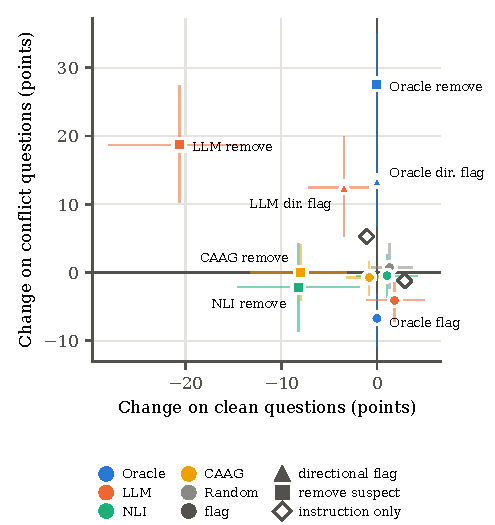
\includegraphics[width=\columnwidth]{generated/fig_tradeoff.pdf}
\caption{Change in one-way strict accuracy on RAMDocs conflict questions (y) against clean questions (x), relative to
no flags (gpt-4o-mini, default skeleton, confirmatory split, 95\% CIs). Colour: detector; shape: format. The oracle
sits on the y-axis because it never flags a clean question. Without direction, removal deletes the second passage of
each pair.}
\label{fig:tradeoff}
\end{figure}

\begin{figure*}[t]
\centering
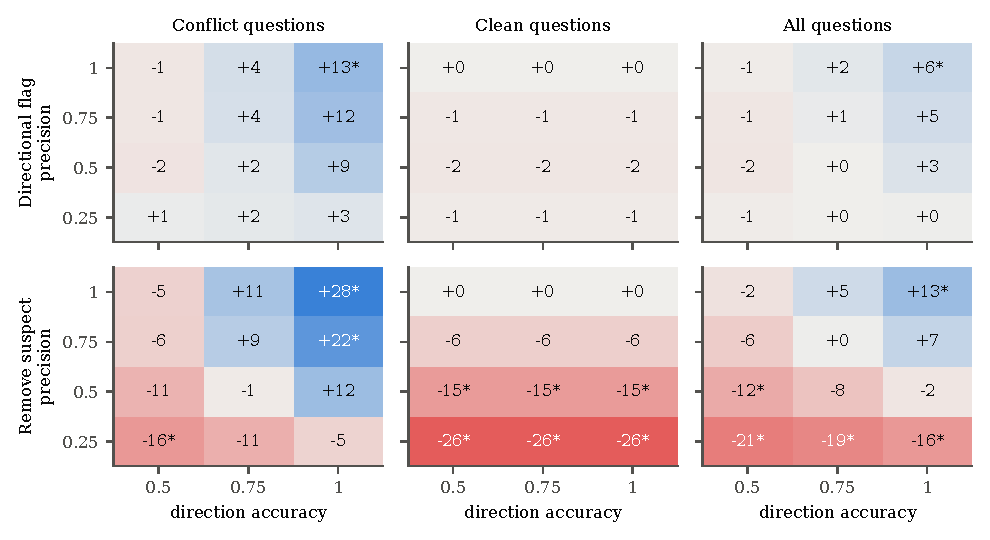
\includegraphics[width=\textwidth]{generated/fig_grid.pdf}
\caption{Synthetic detectors at recall 1: change in one-way strict accuracy (points) against no flags, by pair
precision (rows) and direction accuracy (columns), for the directional flag (top) and removal (bottom). $^*$:
significant after Holm correction over the 36 cells of that format and subset. Clean questions only see false flags,
so their rows do not vary with direction accuracy.}
\label{fig:grid}
\end{figure*}

\paragraph{Construction.}
We build each synthetic detector (Section~\ref{sec:synthetic}) from the gold labels. Each gold contradiction pair is
flagged with probability $r$. False flags are drawn from non-contradicting pairs at a single per-pair rate, set over
the whole split so that expected precision is $p$; clean questions therefore
receive false flags too. A true flag names the gold misinformation side with probability $d$, and otherwise the other side.
A false flag has no misinformation side, so its suspect is picked uniformly. Each pair gets one uniform draw for
flagging and one for direction, and every cell reuses them. Cells are therefore nested: raising $r$ or $d$, or
lowering $p$, only adds flags or corrections, which keeps comparisons across cells paired.

\paragraph{Gains rise with direction accuracy; precision matters mainly for removal.}
Figure~\ref{fig:grid} replaces the oracle with synthetic detectors of known quality. Gains rise with direction
accuracy in both formats. Only the cells with perfect direction are significant on all questions (directional flag
\gDirOneDOneAll, removal \gRemOneDOneAll\ points at perfect precision). Neighbouring cells at direction accuracy
0.75 have similar point estimates on conflict questions, so the pattern is a dose-response, not a threshold. With 36 cells
under Holm, the grid has little power to separate adjacent levels.

Precision matters mainly for removal. On clean questions a cell's prompt does not depend
on direction accuracy, so the false-flag cells reduce to \hFourRemN\ distinct comparisons per format. Removal is
significantly harmful in \hFourRemHarm\ of them, the directional flag in \hFourDirHarm\ (H4a). Under removal, false flags
delete correct passages, which costs clean questions \agRemHalfDOneClean\ points at precision 0.5 and
\agRemQuDOneClean\ at 0.25, while synthetic false directional flags cost at most two points. The harm tracks the
share of clean questions that lose a correct document (Spearman $\rho=\hFourRho$ over \hFourRhoCells\ distinct
cells, 95\% CI \hFourRhoCI\ from a question-level bootstrap; H4b). Removal hurts clean questions significantly more
than the directional flag in \hFourRemWorse\ of \hFourMatched\ matched cells (H4c; we set no threshold, so we report
the count). Removal is both more powerful and more fragile: its best cell gains twice the directional
flag's on all questions, but below precision 0.75 it is the only format that does net harm.


\paragraph{Placing real detectors on the grid.}
\label{sec:placement}
We compare two ways of summarising a real
detector. \emph{Pair-level}: its pair precision, recall and direction accuracy. \emph{Document-level}: what it does
to each subset's documents in a given format. For conflict questions, that is the share whose misinformation documents
are all marked and the share that have a correct document marked; for clean questions, only the latter. Here ``marked'' means removed (remove) or headed as misinformation (directional flag). The prediction
for a subset is the inverse-distance-weighted mean effect of the four nearest grid cells in that space.

\paragraph{Both summaries place most real effects inside the prediction interval.}
Figure~\ref{fig:placement} (Appendix~\ref{app:extra}) tests
whether the grid predicts real detectors' effects (H6). As pre-registered, we bootstrap the whole prediction (cell effects, every detector's
location and the interpolation) over questions, and ask whether the actual effect falls inside the 95\% interval.
Document-level locations put \hSixDocIn\ of \hSixN\ effects inside, and pair-level locations
\hSixPairIn. Document-level errors are smaller on
average (\hSixDocMae\ vs.\ \hSixPairMae\ points), but the paired difference, \hSixMaeDiff\ \hSixMaeDiffCI\ (exact
sign-flip $p=\hSixMaeP$), is not significant over \hSixN\ cases. Both spaces miss the same case, the LLM detector's
removal gain on conflict questions: one correctly directed pair suffices to remove a misinformation document, so the
detector removes the misinformation on \misGoneLlm\% of conflict questions despite its low pair recall. We chose the
document-level axes after seeing the LLM detector on the pilot split. The grid is a useful first estimate of a
detector's effect, but with three detectors we cannot claim that one summary predicts better than the other.

